\chapter{Context-Free Languages \label{chap:kontextfrei}}
In this chapter we present the notion of 
\href{http://en.wikipedia.org/wiki/Context-free_language}{\emph{context-free languages}}.
This concept is much more powerful than the notion of regular languages.  The syntax of most modern
programming languages can be described via context-free languages.  Furthermore, checking whether a
string is a member of a context-free language structures the string into a recursive structure known
as a \emph{parse tree}.  These parse trees are the basis for \emph{understanding} the meaning of a
string that is to be interpreted as a program fragment.  A program that checks whether a given
string is an element of a context-free language is called a \emph{parser}.  Usually, a parser builds
a parse tree from a given string.  Parsing is therefore the first step in an interpreter or a compiler.
In this chapter, we first define the notion of context-free languages.  Next, we discuss parse
trees.  We conclude the chapter by introducing some of the less complex algorithms that are
available for parsing a string into a parse tree.

\section{Kontextfreie Grammatiken \label{kontextfreie}}
Kontextfreie Sprachen dienen zur Beschreibung von Programmier-Sprachen, insofern handelt
es sich bei den kontextfreien Sprachen genau wie bei den regul\"aren Sprachen ebenfalls um
formale Sprachen.  Allerdings wollen wir sp\"ater beim Einlesen eines Programms nicht nur
entscheiden, ob das Programm korrekt ist, sondern wir wollen dar\"uber hinaus den
Programm-Text \emph{strukturieren}.  Den Vorgang des \emph{Strukturierens} bezeichnen wir
auch als \emph{parsen} und das Programm, das diese Strukturierung vornimmt, wird als
\emph{Parser} bezeichnet.  Als Eingabe erh\"alt ein Parser \"ublicherweise nicht den
Text eines Programms, sondern statt dessen eine Folge sogenannter \emph{Terminale}, die auch
als \emph{Token} bezeichnet werden.  Diese 
Token werden von einem Scanner erzeugt, der mit Hilfe regul\"arer Ausdr\"ucke den Programmtext
in einzelne W\"orter aufspaltet, die wir in diesem Zusammenhang als Token bezeichnen.
Beispielsweise spaltet der Scanner des \texttt{C}-Compilers ein \texttt{C}-Programm in die
folgenden Token auf:
\begin{itemize}
\item Operator-Symbole wie ``\texttt{+}'', ``\texttt{+=}'', ``\texttt{<}'',
      ``\texttt{<=}'' etc.,
\item Klammer-Symbole wie ``\texttt{(}'', ``\texttt{[}'', ``\texttt{\{}''  oder
      die schlie{\ss}enden Klammern ``\texttt{)}'', ``\texttt{]}'', ``\texttt{\}}'',
\item vordefinierte Schl\"usselw\"orter wie ``\texttt{if}'', ``\texttt{while}'',
      ``\texttt{typedef}'', ``\texttt{struct}'', etc.,
\item Variablen- und Funktions-Namen wie ``\texttt{x}'', ``\texttt{y}'',
      ``\texttt{printf}'', etc.,
\item Namen f\"ur Typen wie ``\texttt{int}'', ``\texttt{char}'' oder auch benutzerdefinierte
      Typnamen,
\item Literale zur Bezeichnung von Konstanten, wie ``\texttt{1.23}'', 
      ``\texttt{\symbol{34}hallo\symbol{34}}'' oder ``\texttt{\symbol{96}c\symbol{96}}''
\item Kommentare,
\item \emph{White-Space-Zeichen}, (Leerzeichen, Tabulatoren, Zeilenumbr\"uche).
\end{itemize}
Der Parser erh\"alt vom Scanner eine Folge solcher Token und hat die Aufgabe, daraus
einen sogenannten \emph{Syntax-Baum} zu konstruieren.  Dazu bedient sich der Parser einer
\emph{Grammatik}, die mit Hilfe von \emph{Grammatik-Regeln} angibt, wie die Eingabe zu
strukturieren ist.  Betrachten wir als Beispiel das Parsen arithmetischer Ausdr\"ucke.  Die
Menge \textsl{ArithExpr} der arithmetischen Ausdr\"ucke k\"onnen wir induktiv definieren.  
Um die Struktur arithmetischer Ausdr\"ucke korrekt wiedergeben zu k\"onnen, definieren wir
gleichzeitig die Mengen \textsl{Product} und \textsl{Factor}.  
Die Menge \textsl{Product} enth\"alt arithmetische
Ausdr\"ucke, die Produkte und Quotienten darstellen und die Menge \textsl{Factor} enth\"alt
einzelne Faktoren.  Die Definition dieser zus\"atzlichen Mengen ist notwendig, um sp\"ater die
Pr\"azedenzen der Operatoren korrekt darstellen zu k\"onnen.
Die Grundbausteine der arithmetischen Ausdr\"ucke sind Variablen, Zahlen, die
Operator-Symbole 
``\texttt{+}'', ``\texttt{-}'', ``\texttt{*}'', ``\texttt{/}'',
und die Klammer-Symbole ``\texttt{(}'' und ``\texttt{)}''.  Aufbauend auf diesen Symbolen
verl\"auft die induktive Definition der Mengen \textsl{Factor}, \textsl{Product} und
\textsl{ArithExpr} wie folgt:
\begin{enumerate}
\item Jede Zahlenkonstante ist ein Faktor:
      \\[0.2cm]
      \hspace*{1.3cm}
      $C \in \textsl{Number} \Rightarrow C \in \textsl{Factor}$.
\item Jede Variable ist ein Faktor:
      \\[0.2cm]
      \hspace*{1.3cm}
      $V \in \textsl{Variable} \Rightarrow V \in \textsl{Factor}$.
\item Ist $A$ ein arithmetischer Ausdruck und schlie{\ss}en wir diesen Ausdruck in Klammern
      ein, so erhalten wir einen Ausdruck, den wir als Faktor ben\"utzen k\"onnen:
      \\[0.2cm]
      \hspace*{1.3cm}
      $A \in \textsl{ArithExpr} \Rightarrow \quoted{(}A\quoted{)} \in \textsl{Factor}$. 
      \\[0.2cm] 
      Ein Wort zur Notation: W\"ahrend in der obigen Formel $A$ eine Meta-Variable ist, die f\"ur
      einen beliebigen arithmetischen Ausdruck steht, sind die Strings ``\texttt{(}'' 
      und ``\texttt{)}'' w\"ortlich zu interpretieren und 
      deshalb in G\"ansef\"u{\ss}chen eingeschlossen.  Die G\"ansef\"u{\ss}chen sind nat\"urlich nicht Teil
      des arithmetischen 
      Ausdrucks sondern dienen lediglich der Notation.
\item Ist $F$ ein Faktor, so ist $F$ gleichzeitig auch ein Produkt:
      \\[0.2cm]
      \hspace*{1.3cm}
      $F \in \textsl{Factor} \Rightarrow F \in \textsl{Product}$.
\item Ist $P$ ein Produkt und ist $F$ ein Faktor, so sind die Strings 
      $P \quoted{*} F$ und 
      $P \quoted{/} F$ ebenfalls Produkte:
      \\[0.2cm]
      \hspace*{1.3cm}
      $P \in \textsl{Product} \wedge F \in \textsl{Factor} \Rightarrow 
       P \squoted{*} F \in \textsl{Product} \;\wedge\; P \squoted{/} F \in \textsl{Product}$.
\item Jedes Produkt ist gleichzeitig auch ein arithmetischer Ausdruck
      \\[0.2cm]
      \hspace*{1.3cm}
      $P \in \textsl{Product} \Rightarrow P \in \textsl{ArithExpr}$.
\item Ist $A$ ein arithmetischer Ausdruck und ist $P$ ein Produkt, so sind auch
      die Strings $A \quoted{+} P$ und $A \quoted{-} P$  arithmetische Ausdr\"ucke:
      \\[0.2cm]
      \hspace*{1.3cm}
      $A \in \textsl{ArithExpr} \wedge P \in \textsl{Product} \Rightarrow
       A \squoted{+} P \in \textsl{ArithExpr} \;\wedge\; A \squoted{-} P \in \textsl{ArithExpr}$.
\end{enumerate}
Die oben angegebenen Regeln definieren die Mengen \textsl{Factor}, \textsl{Product} und
\textsl{ArithExpr} durch wechselseitige Rekursion.
Diese Definition k\"onnen  wir in Form von sogenannten \emph{Grammatik-Regeln} wesentlich
kompakter schreiben:
\begin{eqnarray*}
  \textsl{arithExpr} & \rightarrow & \textsl{arithExpr} \quoted{+} \textsl{product}  \\
  \textsl{arithExpr} & \rightarrow & \textsl{arithExpr} \quoted{-} \textsl{product}  \\
  \textsl{arithExpr} & \rightarrow & \textsl{product}                                \\[0.1cm]
  \textsl{product}   & \rightarrow & \textsl{product} \quoted{*} \textsl{factor}     \\
  \textsl{product}   & \rightarrow & \textsl{product} \quoted{/} \textsl{factor}     \\
  \textsl{product}   & \rightarrow & \textsl{factor}                                 \\[0.1cm]
  \textsl{factor}    & \rightarrow & \quoted{(} \textsl{arithExpr} \quoted{)}        \\
  \textsl{factor}    & \rightarrow & \textsc{Variable}                               \\
  \textsl{factor}    & \rightarrow & \textsc{Number} 
\end{eqnarray*}
Die Ausdr\"ucke auf der linken Seite einer Grammatik-Regel bezeichnen wir als
\emph{syntaktische Variablen} oder auch als \emph{Nicht-Terminale}.  
Wir werden syntaktische Variablen \"ublicherweise klein schreiben, denn das ist die Konvention
bei den  Parser-Generatoren \textsc{Antlr} und \textsl{JavaCup}, die wir sp\"ater vorstellen werden. 
In der Literatur ist es allerdings oft anders herum.  Dort werden die syntaktischen Variablen gro{\ss} und
die \emph{Terminale}  klein geschrieben.  Gelegentlich wird eine
syntaktische Variable auch als eine \emph{syntaktische Kategorie} bezeichnet.
 
In dem Beispiel sind \textsl{arithExpr}, \textsl{product} und \textsl{factor} die 
syntaktischen Variablen.  Die restlichen Ausdr\"ucke, in unserem Fall also \textsc{Number}, \textsc{Variable} und
die Zeichen 
``\texttt{+}'', ``\texttt{-}'', ``\texttt{*}'', ``\texttt{/}'', ``\texttt{(}'' und ``\texttt{)}''
bezeichnen wir als \emph{Terminale} oder auch \emph{Token}.  Dies sind also genau die
Zeichen, die nicht auf der linken Seite einer Grammatik-Regel stehen.
Bei den Nicht-Terminalen gibt es zwei Arten:
\begin{enumerate}
\item Operator-Symbole und Trennzeichen wie beispielsweise ``\texttt{/}'' und
      ``\texttt{(}''.  

      Solche Nicht-Terminalen stehen f\"ur sich selbst.
\item Token wie \textsc{Number} oder \textsc{Variable} ist zus\"atzlich ein Wert zugeordnet.
      Im Falle von \textsc{Number} ist dies eine Zahl, im Falle von \textsc{Variable}
      ist dies ein String, der den Namen der Variablen wiedergibt.  Diese Art von Token werden wir
      zur besseren Unterscheidung von den Variablen immer mit Gro{\ss}buchstaben schreiben.
      Damit folgen wir der Praxis von Parser-Generatoren wie \textsc{Antlr} und \textsl{JavaCup}.
\end{enumerate}
\"Ublicherweise werden Grammatik-Regeln in einer kompakteren Notation als der oben vorgestellten
wiedergegeben, indem alle Regeln f\"ur ein Nicht-Terminal zusammengefasst werden.  F\"ur unser Beispiel
sieht das dann wie folgt aus:
\begin{eqnarray*}
  \textsl{arithExpr} & \rightarrow & \textsl{arithExpr} \quoted{+} \textsl{product} \;\mid\;
                                     \textsl{arithExpr} \quoted{-} \textsl{product} \;\mid\; 
                                     \textsl{product}                                            \\
  \textsl{product}   & \rightarrow & \textsl{product} \quoted{*} \textsl{factor} \;\mid\;
                                     \textsl{product} \quoted{/} \textsl{factor} \;\mid\;
                                     \textsl{factor}                                             \\
  \textsl{factor}    & \rightarrow & \squoted{(}\, \textsl{arithExpr} \quoted{)} \;\mid\; 
                                     \textsc{Number} \;\mid\; \textsc{Variable}
\end{eqnarray*}
Hier werden also die einzelnen Alternativen einer Regel durch das Metazeichen \squoted{|}
getrennt.  Nach dem obigen Beispiel geben wir jetzt die formale Definition f\"ur den Begriff der
\href{http://en.wikipedia.org/wiki/Context-free_grammar}{kontextfreien Grammatik}.

\begin{Definition}[Kontextfreie Grammatik]
Eine \emph{kontextfreie Grammatik} $G$ ist ein 4-Tupel 
\[ 
   G = \langle V, T, R, S \rangle,
\]
so dass folgendes gilt:
\begin{enumerate}
\item $V$ ist eine Menge von Namen, die wir als \emph{syntaktische Variablen} oder auch
      \emph{Nicht-Terminale} bezeichnen. 
      
      In dem obigen Beispiel gilt 
      \\[0.2cm]
      \hspace*{1.3cm}
      $V = \{ \textsl{arithExpr}, \textsl{product}, \textsl{factor} \}$.
\item $T$ ist eine Menge von Namen, die wir als \emph{Terminale} bezeichnen.  
      Die Mengen $T$ und $V$ sind disjunkt, es gilt also
      \\[0.2cm]
      \hspace*{1.3cm}
      $T \cap V = \emptyset$.
      \\[0.2cm]
      In dem obigen Beispiel gilt
      \\[0.2cm]
      \hspace*{1.3cm}
      $T = \{ \textsc{Number}, \textsc{Variable}, \quoted{+}, \quoted{-}, \quoted{*}, \quoted{/}, \quoted{(}, \quoted{)} \}$
\item $R$ ist die Menge der Regeln.  Formal ist eine Regel ein Paar $\langle A, \alpha \rangle$:
      \begin{enumerate}
      \item Die erste Komponente dieses Paares ist eine syntaktische Variable:
            \\[0.2cm]
            \hspace*{1.3cm}
            $A \in V$.
      \item Die zweite Komponente ist ein String, der aus syntaktischen Variablen und 
            Terminalen aufgebaut ist:
            \\[0.2cm]
            \hspace*{1.3cm}
            $\alpha \in (V \cup T)^*$.
      \end{enumerate}
      Insgesamt gilt  f\"ur die Menge der Regeln $R$ damit
      \\[0.2cm]
      \hspace*{1.3cm}
      $R \subseteq V \times (V \cup T)^*$
      
      Ist $\langle x, \alpha \rangle$ eine Regel, so schreiben wir diese Regel als
      \\[0.2cm]
      \hspace*{1.3cm}
      $x \rightarrow \alpha$.
      \\[0.2cm]
      Beispielsweise haben wir oben die erste Regel als
      \\[0.2cm]
      \hspace*{1.3cm}
      $\textsl{arithExpr} \rightarrow \textsl{arithExpr} \quoted{+} \textsl{product}$
      \\[0.2cm]
      geschrieben.  Formal steht diese Regel f\"ur das Paar
      \\[0.2cm]
      \hspace*{1.3cm}
      $\bigl\langle \textsl{arithExpr}, [\textsl{arithExpr}, \squoted{+}, \textsl{product}] \bigr\rangle$. 
\item $S$ ist ein Element der Menge $V$, das wir als das \emph{Start-Symbol} bezeichnen. 
      In dem obigen Beispiel ist \textsl{arithExpr} das Start-Symbol.
      \qed
\end{enumerate}
\end{Definition}

\subsection{Ableitungen}
Als n\"achstes wollen wir festlegen, welche Sprache durch eine gegebene Grammatik $G$ definiert wird.
Dazu definieren wir zun\"achst den Begriff eines \emph{Ableitungs-Schrittes}.  Es sei
\begin{enumerate}
\item $G = \langle V, T, R, S \rangle$ eine Grammatik,
\item $a \in V$ eine syntaktische Variable,
\item $\alpha a \beta \in (V \cup T)^*$ ein String aus Terminalen und syntaktischen Variablen,
      der die Variable $a$ enth\"alt,
\item $(a \rightarrow \gamma) \in R$ eine Regel.
\end{enumerate}
Dann kann der String $\alpha a \beta$ durch einen Ableitungs-Schritt in den String 
$\alpha \gamma \beta$ \"uberf\"uhrt werden, wir ersetzen also ein Auftreten der syntaktische Variable
$a$ durch die rechte Seite der Regel $a \rightarrow \gamma$.  Diesen Ableitungs-Schritt schreiben
wir als
\\[0.2cm]
\hspace*{1.3cm}
$\alpha a \beta \Rightarrow_G \alpha \gamma \beta$.
\\[0.2cm]
Geht die verwendete Grammatik $G$ aus dem Zusammenhang klar hervor, so wird der Index $_G$
weggelassen und wir schreiben k\"urzer $\Rightarrow$ an Stelle von $\Rightarrow_G$.
Der transitive und reflexive Abschluss der Relation $\Rightarrow_G$ wird mit $\Rightarrow_G^*$
bezeichnet.  Wollen wir ausdr\"ucken, dass die Ableitung des Strings $w$ aus dem
Nicht-Terminal $a$ aus $n$ Ableitungs-Schritten
besteht, so schreiben wir 
\\[0.2cm]
\hspace*{1.3cm}
$a \Rightarrow^n w$.
\\[0.2cm]  
Wir geben ein Beispiel:
\begin{eqnarray*}
\textsl{arithExpr} 
& \Rightarrow & \textsl{arithExpr} \quoted{+} \textsl{product}  \\
& \Rightarrow & \textsl{product} \quoted{+} \textsl{product}  \\
& \Rightarrow & \textsl{product} \quoted{*} \textsl{factor} \quoted{+} \textsl{product} \\
& \Rightarrow & \textsl{factor} \quoted{*} \textsl{factor} \quoted{+} \textsl{product}  \\
& \Rightarrow & \textsc{Number} \quoted{*} \textsl{factor} \quoted{+} \textsl{product}  \\
& \Rightarrow & \textsc{Number} \quoted{*} \textsc{Number} \quoted{+} \textsl{product}  \\
& \Rightarrow & \textsc{Number} \quoted{*} \textsc{Number} \quoted{+} \textsl{factor}   \\
& \Rightarrow & \textsc{Number} \quoted{*} \textsc{Number} \quoted{+} \textsc{Number}   
\end{eqnarray*}
Damit haben wir also gezeigt, dass
\\[0.2cm]
\hspace*{1.3cm}
$\textsl{arithExpr} \Rightarrow^* \textsc{Number} \quoted{*} \textsc{Number} \quoted{+} \textsc{Number}$
\\[0.2cm]
oder genauer
\\[0.2cm]
\hspace*{1.3cm}
$\textsl{arithExpr} \Rightarrow^8 \textsc{Number} \quoted{*} \textsc{Number} \quoted{+} \textsc{Number}$
\\[0.2cm]
gilt.  Ersetzen wir hier das Terminal \textsc{Number} durch verschiedene Zahlen, so haben wir damit
beispielsweise gezeigt, dass der String
\\[0.2cm]
\hspace*{1.3cm}
$2 * 3 + 4$
\\[0.2cm]
ein arithmetischer Ausdruck ist.  Allgemein definieren wir die durch eine Grammatik $G$ definierte
Sprache $L(G)$ als die Menge aller Strings, die einerseits nur aus Terminalen bestehen und die sich
andererseits aus dem Start-Symbol $S$ der Grammatik ableiten lassen:
\\[0.2cm]
\hspace*{1.3cm}
$L(G) := \bigl\{ w \in T^* \mid S \Rightarrow^* w \bigr\}$.


\example
Die Sprache
\\[0.2cm]
\hspace*{1.3cm}
$L = \{ (^n )^n \mid n \in \mathbb{N}_0 \}$ 
\\[0.2cm]
wird von der Grammatik 
\\[0.2cm]
\hspace*{1.3cm}
$G = \bigl\langle \{s\}, \{ \squoted{(}, \squoted{)} \}, R, \textsl{s} \bigr\rangle$
\\[0.2cm]
erzeugt, wobei die Regeln $R$ wie folgt gegeben sind:
\\[0.2cm]
\hspace*{1.3cm}
$\textsl{s} \rightarrow \quoted{(} \textsl{s} \quoted{)}  \mid  \varepsilon$.





\proof
Wir zeigen zun\"achst, dass sich jedes Wort $w \in L$ aus dem
Start-Symbol $\textsl{s}$ ableiten l\"asst:
\\[0.2cm]
\hspace*{1.3cm}
$w \in L \;\Longrightarrow\; \textsl{s} \Rightarrow^* w$.
\\[0.2cm]
Es sei also $w_n = (^n)^n$.  Wir zeigen durch Induktion \"uber $n \in \mathbb{N}_0$, dass $w_n \in L(G)$ ist.
\begin{enumerate}
\item[I.A.:] $n=0$.
  
            Es gilt $w_0 = \varepsilon$.  Offenbar haben wir
            \\[0.2cm]
            \hspace*{1.3cm}
            $\textsl{s} \Rightarrow \varepsilon$,
            \\[0.2cm]
            denn die Grammatik enth\"alt die Regel $s \rightarrow \varepsilon$.
            Also gilt $w_0 \in L(G)$.
\item[I.S.:] $n \mapsto n + 1$. 

            Der String $w_{n+1}$ hat die Form $w_{n+1} = \quoted{(}w_n\quoted{)}$, wobei
            der String $w_n$ nat\"urlich ebenfalls in $L$ liegt.
            Also gibt es nach I.V. eine Ableitung von $w_n$:
            \\[0.2cm]
            \hspace*{1.3cm}
            $\textsl{s} \Rightarrow^* w_n$.
            \\[0.2cm]
            Insgesamt haben wir dann die Ableitung
            \\[0.2cm]
            \hspace*{1.3cm}
            $\textsl{s} \Rightarrow \quoted{(}\textsl{s}\quoted{)} \Rightarrow^* \quoted{(} w_n \quoted{)} = w_{n+1}$.
            \\[0.2cm]
            Also gilt  $w_{n+1} \in L(G)$.
\end{enumerate}
Als n\"achstes zeigen wir, dass jedes Wort $w$, das sich aus $\textsl{s}$ ableiten l\"asst, ein Element
der Sprache $L$ ist.  Wir f\"uhren den Beweis durch Induktion \"uber die Anzahl $n \in \mathbb{N}$ der
Ableitungs-Schritte:
\begin{enumerate}
\item[I.A.:] $n = 1$.
  
            Die einzige Ableitung eines aus Terminalen aufgebauten Strings, die nur aus 
            einem Schritt besteht, ist
            \\[0.2cm]
            \hspace*{1.3cm}
            $\textsl{s} \Rightarrow \varepsilon$.
            \\[0.2cm]
            Folglich muss $w = \varepsilon$ gelten und wegen $\varepsilon = (^0)^0 \in L$
            haben wir $w \in L$.
\item[I.S.:] $n \mapsto n+1$.

            Wenn die Ableitung aus mehr als einem Schritt besteht, dann muss die Ableitung
            die folgende Form haben:
            \\[0.2cm]
            \hspace*{1.3cm}
            $\textsl{s} \Rightarrow \quoted{(} \textsl{s} \quoted{)} \Rightarrow^n w$
            \\[0.2cm]
            Daraus folgt
            \\[0.2cm]
            \hspace*{1.3cm}
            $w = \quoted{(}v\quoted{)} \;\wedge\; \textsl{s} \Rightarrow^n v$.
            \\[0.2cm]
            Nach I.V.~gilt dann $v \in L$.  Damit gibt es $k \in \mathbb{N}_0$ mit $v = (^k)^k$.
            Also haben wir
            \\[0.2cm]
            \hspace*{1.3cm}
            $w = \quoted{(}v\quoted{)} = 
((^k)^k) = (^{k+1})^{k+1} \in L$. \qed
\end{enumerate}


\exercise
Wir definieren f\"ur $w \in \Sigma^*$ und $c \in \Sigma$ die Funktion
\\[0.2cm]
\hspace*{1.3cm}
$\textsl{count}(w,c)$,
\\[0.2cm]
die z\"ahlt, wie oft der Buchstabe $c$ in dem Wort $w$ vorkommt, durch Induktion \"uber $w$.
\begin{enumerate}
\item[I.A.:] $w = \varepsilon$.  

            Wir setzen
            \\[0.2cm]
            \hspace*{1.3cm}
            $\textsl{count}(\varepsilon, c) := 0$.
\item[I.S.:] $w = dv$ mit $d \in \Sigma$ und $v \in \Sigma^*$.  

            Dann wird $\textsl{count}(dv,c)$ durch eine Fall-Unterscheidung definiert:
            \\[0.2cm]
            \hspace*{1.3cm}
            $\textsl{count}(dv,c) := \left\{
             \begin{array}[c]{llr}
               \textsl{count}(v,c) + 1 & \mbox{falls $c     = d$}; \\
               \textsl{count}(v,c)     & \mbox{falls $c \not= d$}. \\
             \end{array}\right.
            $ \eox
\end{enumerate}
Wir setzen nun $\Sigma = \{ \squoted{A}, \squoted{B} \}$ und definieren die Sprache $L$ als die
Menge der W\"orter $w\in\Sigma^*$, in denen die Buchstaben \squoted{A} und \squoted{B} mit der
selben H\"aufigkeit vorkommen:
\\[0.2cm]
\hspace*{1.3cm}
$L := \bigl\{ w \in \Sigma^* \mid \textsl{count}(w,\squoted{A}) = \textsl{count}(w,\squoted{B})\bigr\}$
\\[0.2cm]
Geben Sie eine Grammatik $G$ an, so dass $L = L(G)$ gilt und beweisen Sie Ihre Behauptung!
\eox

\exerciseEng
Define $\Sigma := \{ \squoted{A}, \squoted{B} \}$. 
In the previous chapter, we have already defined the reversal of a string 
$w = c_1 c_2 \cdots c_{n-1} c_n \in \Sigma^*$ as the string
\\[0.2cm]
\hspace*{1.3cm}
$w^R := c_n c_{n-1} \cdots c_2 c_1$.
\\[0.2cm]
A string $w \in \Sigma^*$ is called a
\href{http://en.wikipedia.org/wiki/Palindrome}{\emph{palindrome}} if the string is identical to its
reversal, i.e.~if
\\[0.2cm]
\hspace*{1.3cm}
$w = w^R$
\\[0.2cm]
holds true.  For example, the strings 
\\[0.2cm]
\hspace*{1.3cm}
$w_1 = \mathtt{ABABA}$ \quad and \quad $w_2 = \mathtt{ABBA}$
\\[0.2cm]
are both palindromes, while the string \texttt{ABB} is not a palindrome. The 
\emph{language of palindromes} $L_\mathrm{palindrome}$ is the set of all 
strings in $\Sigma^*$ that are palindromes, i.e.~we have
\\[0.2cm]
\hspace*{1.3cm}
$L_\mathrm{palindrome} := \bigr\{ w \in \Sigma^* \mid w = w^R \bigr\}$.
\renewcommand{\labelenumi}{(\alph{enumi})}
\begin{enumerate}
\item Prove that the language $L_\mathrm{palindrome}$ is a context-free language.
\item Prove that the language $L_\mathrm{palindrome}$ is not regular.  \eox
\end{enumerate}
\renewcommand{\labelenumi}{\arabic{enumi}.}

 

\exerciseStar
Es sei $\Sigma := \{ \squoted{A}, \squoted{B} \}$.  Wir definieren die Menge $L$ als die
Menge der Strings $s$, die sich \underline{nicht} in der Form $s = ww$ schreiben lassen:
\\[0.2cm]
\hspace*{1.3cm}
$L = \bigl\{ s \in \Sigma^* \mid \neg(\exists w\in\Sigma^*: s = ww)\bigr\}$.
\\[0.2cm]
Geben Sie eine kontextfreie Grammatik $G$ an, die diese Sprache erzeugt.
\eox

\solution 
Die L\"osung dieser Aufgabe ist so umfangreich, dass wir unsere \"Uberlegungen in vier Teile aufspalten.
\vspace{0.2cm}

\noindent
\textbf{Vor\"uberlegung \texttt{I}}: String-Notationen \\
F\"ur einen String $s$ bezeichnen wir mit $s[i]$ den $i$-ten Buchstaben und mit
$s[i\!:\!j]$ den Teilstring, der sich vom $i$-ten Buchstaben bis zum $j$-ten Buchstaben einschlie{\ss}lich
erstreckt.  Bei der Nummerierung beginnen wir mit 1.
Dann gilt
\begin{enumerate}
\item $|s[i\!:\!j]| = j - i + 1$

      Von der Notwendigkeit, hier eine 1 zu addieren, k\"onnen wir uns dadurch \"uberzeugen, wenn wir den
      Fall $i = j$ betrachten, denn $s[i\!:\!i]$ ist der Teilstring, der nur aus dem $i$-ten
      Buchstaben besteht und der hat nat\"urlich die L\"ange 1.
\item $s[i\!:\!j][k] = s[i + k - 1]$.

      Dass in diesem Fall 1 subtrahiert werden muss, sehen Sie, wenn Sie den Fall $k=1$ betrachten,
      denn der erste Buchstabe des Teilstrings $s[i\!:\!j]$ ist nat\"urlich der $i$-te
      Buchstabe von $s$.
\item Hat ein Wort $s \in \Sigma^*$ eine ungerade L\"ange, gilt also
      \\[0.2cm]
      \hspace*{1.3cm}
      $|s| = 2 \cdot n +1$ \quad f\"ur ein $n \in \mathbb{N}_0$,
      \\[0.2cm]
      so liegt der Buchstabe $s[n + 1]$ in der Mitte von $s$.  Um dies einzusehen,
      betrachten wir die Teilstrings $s[1:n]$ und $s[n+2:2\cdot n+1]$, die links und rechts
      von $s[n+1]$ liegen:
      \\[0.2cm]
      \hspace*{1.3cm}
      $\underbrace{s[1] \cdots s[n]}_{s[1:n]} s[n+1] \underbrace{s[n+2] \cdots s[2 \cdot n
        +1]}_{s[n+2:2\cdot n+1]}$
      \\[0.2cm]
      Offenbar sind diese Teilstrings gleich lang, denn wir haben
      \\[0.2cm]
      \hspace*{1.3cm}
      $|s[1:n]| = n$ \quad und \quad $|s[n+2:2\cdot n+1]| = 2 \cdot n + 1 - (n+2) + 1 = n$.
      \\[0.2cm]
      Also liegt der Buchstabe $s[n+1]$ tats\"achlich in der Mitte von $s$.  

      F\"ur einen String $s$ ungerader L\"ange definieren wir $\hat{s}$ als den Buchstaben,
      der in der Mitte von $s$ liegt:
      \\[0.2cm]
      \hspace*{1.3cm}
      $\hat{s} := s[n+1]$ \quad falls $|s| = 2 \cdot n + 1$.
\end{enumerate}

\noindent
\textbf{Vor\"uberlegung \texttt{II}}:
Zun\"achst ist klar, dass alle Strings deren L\"angen ungerade sind, in der Sprache $L$ liegen,
denn jeder String der Form $s=ww$ hat offenbar die L\"ange 
\\[0.2cm]
\hspace*{1.3cm}
$|s| = |w| + |w| = 2\cdot |w|$
\\[0.2cm]
und das ist eine gerade Zahl.

Gilt nun $s \in L$ mit $|s| = 2 \cdot n$, so l\"asst sich $s$ in zwei Teile $u$ und $v$ gleicher
L\"ange zerlegen:
\\[0.2cm]
\hspace*{1.3cm}
$s = uv \quad \mbox{mit} \quad u = s[1\!:\!n], \quad v = s[n+1\!:\!2 \cdot n]
  \quad \mbox{und} \quad u \not= v
$.
\\[0.2cm]
Aus der Ungleichung $u \not= v$ folgt, dass es mindestens einen Index $k \in \{1,\cdots,n\}$ gibt,
so dass sich die Strings $u$ und $v$ an diesem Index unterscheiden:
\\[0.2cm]
\hspace*{1.3cm}
$u[k] \not= v[k]$. 
\\[0.2cm]
Der Trick besteht jetzt darin, den String $s$ in zwei Teilstrings $x$ und $y$ aufzuteilen,
von denen der eine 
Teilstring in der Mitte den Buchstaben $u[k]$ enth\"alt, w\"ahrend der andere Teilstring in der Mitte den
Buchstaben $v[k]$ enth\"alt.  Wir definieren
\\[0.2cm]
\hspace*{1.3cm}
$x := s[1\!:\!2 \cdot k - 1] \quad \mbox{und} \quad y := s[2 \cdot k\!:\! 2 \cdot n]$.
\\[0.2cm]
F\"ur die L\"angen von $x$ und $y$ folgt daraus
\\[0.2cm]
\hspace*{1.3cm}
$|x| = 2 \cdot k - 1 \quad \mbox{und} \quad |y| = 2 \cdot (n - k) + 1$. 
\\[0.2cm]
Dann gilt einerseits
\\[0.2cm]
\hspace*{1.3cm}
$x[k] = s[k] = u[k]$
\\[0.2cm]
und andererseits haben wir
\\[0.2cm]
\hspace*{1.3cm}
$
\begin{array}[t]{lcl}
    y[n - k + 1] & = & s[2 \cdot k\!:\! 2 \cdot n][n - k + 1] \\[0.1cm]
                 & = & s[2 \cdot k + (n - k + 1) - 1]     \\[0.1cm]
                 & = & s[n + k]                           \\[0.1cm]
                 & = & s[n+1\!:\! 2 \cdot n][k]               \\[0.1cm]
                 & = & v[k]               
\end{array}
$
\\[0.2cm]
Die beiden Buchstaben $u[k]$ und $v[k]$, die daf\"ur verantwortlich sind, dass $u$ und $v$ verschieden
sind, befinden sich also genau in der Mitte der Strings $x$ und $y$.
\vspace{0.3cm}

\noindent
\textbf{Bemerkung}: Wir haben soeben Folgendes gezeigt:  Falls $s \in L$ mit $|s| = 2 \cdot n$ ist, so l\"asst
sich $s$ so in zwei Strings $x$ und $y$ aufspalten, dass die Buchstaben, die jeweils in
der Mitte von $x$ und $y$ liegen, unterschiedlich sind:
\\[0.2cm]
\hspace*{1.3cm}
$s \in L \wedge |s| = 2 \cdot n \rightarrow \exists x,y \in \Sigma^*: \bigl(
 s = xy \wedge \hat{x} \not= \hat{y}\bigr)$.
\vspace{0.3cm}

\noindent
\textbf{Vor\"uberlegung \texttt{III}}:
Wir \"uberlegen uns nun, dass auch die Umkehrung des in der letzten Bemerkung angegebenen
Zusammenhangs gilt:  Sind $x, y \in \Sigma^*$ mit ungerader L\"ange und gilt 
$\hat{x} \not= \hat{y}$, so liegt der String $xy$ in der Sprache $L$:
\\[0.2cm]
\hspace*{1.3cm}
$x, y \in \Sigma^* \wedge |x| = 2 \cdot m + 1 \wedge |y| = 2 \cdot n + 1 \wedge \hat{x}
\not= \hat{y} \rightarrow xy \in L$. \hspace*{\fill} $(*)$
\\[0.2cm]

\noindent
\textbf{Beweis}: Wir definieren $s$ als die Konkatenation von $x$ und $y$, also $s := xy$.
F\"ur die L\"ange von $s$ gilt dann
\\[0.2cm]
\hspace*{1.3cm}
$|s| = 2 \cdot (m + n + 1)$.
\\[0.2cm]
Wir werden zeigen, dass
\\[0.2cm]
\hspace*{1.3cm}
$s[m+1] \not= s[(m+n+1) + (m+1)]$
\\[0.2cm]
gilt.  Spalten wir $s$ in zwei gleich lange Teile $u$ und $v$ auf, definieren also 
\\[0.2cm]
\hspace*{1.3cm}
$u := s[1:m+n+1]$ \quad und \quad
$v := s[m+n+2: 2\cdot(m+n+1)]$, 
\\[0.2cm]
so werden wir gleich sehen, dass
\\[0.2cm]
\hspace*{1.3cm}
$u[m+1] = s[m+1] \not= s[(m+n+1) + (m+1)] = v[m+1]$,
\\[0.2cm]
gilt, woraus  $u \not= v$ und damit $s = uv \in L$ folgt. 
\vspace{0.3cm}

\noindent
Es bleibt der Nachweis von  $s[m+1] \not= s[(m+n+1) + (m+1)]$ zu erledigen:
\\[0.2cm]
\hspace*{1.3cm}
$
\begin{array}[t]{lcll}
  s[(m+n+1) + m + 1] &     = & (xy)[(m+n+1) + m + 1]  & \mbox{wegen $s = xy$} \\
                     &     = & y[n+1]  & \mbox{denn $|x| = 2 \cdot m + 1$}    \\
                     &     = & \hat{y} & \mbox{denn $|y| = 2 \cdot n + 1$}    \\
                     & \not= & \hat{x}                                        \\
                     &     = & x[m+1]  & \mbox{denn $|x| = 2 \cdot m + 1$}    \\
                     &     = & s[m+1]  & \mbox{wegen $s = xy$}.
\end{array}
$
\\[0.2cm]
Damit ist der Beweis der Behauptung $(*)$ abgeschlossen.
\vspace{0.2cm}

\noindent
\textbf{Aufstellen der Grammatik}:
Fassen wir die letzten beiden Vor\"uberlegungen zusammen, so stellen wir fest, dass die
Sprache $L$ aus genau den W\"ortern besteht, die entweder 
eine ungerade L\"ange haben, oder die aus Paaren von Strings ungerader L\"ange bestehen, die
in der Mitte unterschiedliche Buchstaben haben:
\\[0.2cm]
\hspace*{1.3cm}
$\begin{array}[t]{lcl}
  L & =    & \bigl\{ s \in \Sigma^* \big|\; |s| \,\texttt{\%}\, 2 = 1 \bigr\}  \\[0.1cm]
    & \cup & \bigl\{ s \in \Sigma^* \big|\; \exists x,y \in \Sigma^*: 
                             s = xy \wedge |x| \,\texttt{\%}\, 2 = 1 
                                    \wedge |y| \,\texttt{\%}\, 2 = 1  \wedge \hat{x} \not= \hat{y} \bigr\} 
 \end{array}$
\\[0.2cm]
Damit l\"asst sich die Menge $L$ durch die folgende Grammatik beschreiben
\\[0.2cm]
\hspace*{1.3cm}
$G = \langle \{ s, a, b, x, u \}, \{ \squoted{A}, \squoted{B} \}, R, s \rangle$,
\\[0.2cm]
wobei die Menge der Regeln wie folgt gegeben ist:
\\[0.2cm]
\hspace*{1.3cm}
$ 
\begin{array}[t]{lcl}
  s & \rightarrow & u \mid a b \mid  b a \\[0.3cm]
  a & \rightarrow & \squoted{A} \mid x a x         \\[0.3cm]
  b & \rightarrow & \squoted{B} \mid x b x         \\[0.3cm]
  u & \rightarrow & x \mid u x x         \\[0.3cm]
  x & \rightarrow & \squoted{A} \mid \squoted{B}
\end{array}$
\\[0.2cm]
Wir diskutieren die verschiedenen syntaktischen Variablen.
\begin{enumerate}
\item $L(x) = \{ \squoted{A}, \squoted{B} \}$.
\item $L(u) = \{ w \in \Sigma^* \mid \;|w| \,\texttt{\%}\, 2 = 1 \}$,

      denn ein String ungerader L\"ange hat entweder die L\"ange 1 oder er kann aus einem String ungerader L\"ange
      durch Anf\"ugen zweier Buchstaben erzeugt werden.
\item $L(a) = \{ w \in \Sigma^* \mid\; \exists k \in \mathbb{N}: |w| = 2 \cdot k - 1 \wedge w[k] = \squoted{A} \}$,
  
      denn wenn wir an einen String, bei dem der Buchstabe $\squoted{A}$ in der Mitte steht, vorne
      und hinten jeweils einen Buchstaben anf\"ugen, erhalten wir wieder einen String, in
      dessen Mitte der Buchstabe $\squoted{A}$ steht
\item $L(b) = \{ w \in \Sigma^* \mid\; \exists k \in \mathbb{N}: |w| = 2 \cdot k - 1 \wedge w[k] = \squoted{B} \}$,

      denn die Variable $b$ ist analog zur Variablen $a$ definiert worden.  Der einzige
      Unterschied ist der, dass nun der Buchstabe $B$ in der Mitte liegt.
\item $
  \begin{array}[t]{lcl}    
L(s) & = & \quad \bigl\{ w \in \Sigma^* \big|\; |w| \,\texttt{\%}\, 2 = 1 \bigr\} \\[0.1cm] 
     &   & \cup\; \bigl\{ w \in \Sigma^* \big|\; \exists x,y \in \Sigma^*: 
                          w = xy \wedge |x| \,\texttt{\%}\, 2 = 1 
                                 \wedge |y| \,\texttt{\%}\, 2 = 1  \wedge \hat{x} \not= \hat{y} \bigr\} \\[0.2cm]
     & = & \quad \bigl\{ w \in \Sigma^* \mid \neg (\exists v \in \Sigma^*: w = vv) \bigr\}
  \end{array}
$
      \\[0.2cm]
      denn wir haben oben argumentiert, dass alle Strings der Sprache $L$ entweder eine
      ungerade L\"ange haben oder in zwei Teile ungerader L\"ange zerlegt werden k\"onnen, so dass in der Mitte
      dieser Teile verschiedene Buchstaben stehen: Entweder steht im ersten Teil ein $\squoted{A}$
      und im zweiten Teil steht ein $\squoted{B}$ oder es ist umgekehrt.
\end{enumerate}
Um die obigen Behauptungen formal zu beweisen m\"ussten wir nun einerseits noch durch eine Induktion
nach der L\"ange der Herleitung zeigen, dass die von den Grammatik-Symbolen erzeugten
Strings tats\"achlich in den oben angegebenen Mengen liegen.  Andererseits m\"ussten wir f\"ur
die oben angegebenen Mengen zeigen, dass sich jeder String der jeweiligen Menge auch tats\"achlich mit den
angegebenen Grammatik-Regeln erzeugen l\"asst.  Dieser Nachweis w\"urde dann durch Induktion \"uber die L\"ange der
einzelnen Strings gef\"uhrt werden.  Da diese Nachweise einfach sind und keine
\"Uberraschungen mehr bieten, verzichten wir hier darauf.
\qed

\remark
Wir werden sp\"ater sehen, dass das Komplement der in der letzten Aufgabe definierten Sprache $L$,
also die Sprache
\\[0.2cm]
\hspace*{1.3cm}
$L^\mathtt{c} := \Sigma^* \backslash L = \bigl\{ ww \mid  w\in\Sigma^* \bigr\}$
\\[0.2cm]
keine kontextfreie Sprache ist.  Damit sehen wir dann, dass die Menge der kontextfreien Sprachen
nicht unter Komplementbildung abgeschlossen ist. \eox

\subsection{Parse-B\"aume}
Mit Hilfe einer Grammatik $G$ k\"onnen wir nicht nur erkennen, ob ein gegebener String $s$ ein
Element der von der Grammatik erzeugten Sprache $L(G)$ ist, wir k\"onnen den String auch
\emph{strukturieren} indem wir einen \emph{Parse-Baum} aufbauen.  Ist eine Grammatik
\\[0.2cm]
\hspace*{1.3cm}
$G = \langle V, T, R, S \rangle$
\\[0.2cm]
gegeben, so ist ein Parse-Baum f\"ur diese Grammatik ein Baum, der den folgenden 
Bedingungen gen\"ugt:
\begin{enumerate}
\item Jeder innere Knoten (also jeder Knoten, der kein Blatt ist),
      ist mit einer Variablen beschriftet.
\item Jedes Blatt ist mit einem Terminal oder mit einer Variablen beschriftet.
\item Falls ein Blatt mit einer Variablen $a$ beschriftet ist, dann enth\"alt die Grammatik eine 
      Regel der Form
      \\[0.2cm]
      \hspace*{1.3cm}
      $a \rightarrow \varepsilon$.
\item Ist ein innerer Knoten mit einer Variablen $a$ beschriftet und sind die Kinder
      dieses Knotens mit den Symbolen $X_1$, $X_2$, $\cdots$, $X_n$ beschriftet, so
      enth\"alt die Grammatik $G$ eine Regel der Form 
      \\[0.2cm]
      \hspace*{1.3cm}
      $a \rightarrow X_1 X_2 \cdots X_n$.
\end{enumerate}
Die Bl\"atter des Parse-Baums ergeben dann, wenn wir sie von links nach rechts lesen, ein Wort,
das von der Grammatik $G$ abgeleitet wird.  Abbildung \ref{fig:parse-tree.dot} zeigt einen
Parse-Baum f\"ur das Wort ``\texttt{2*3+4}'', der mit der oben angegebenen Grammatik f\"ur
arithmetische Ausdr\"ucke abgeleitet worden ist.

\begin{figure}[!ht]
  \centering
      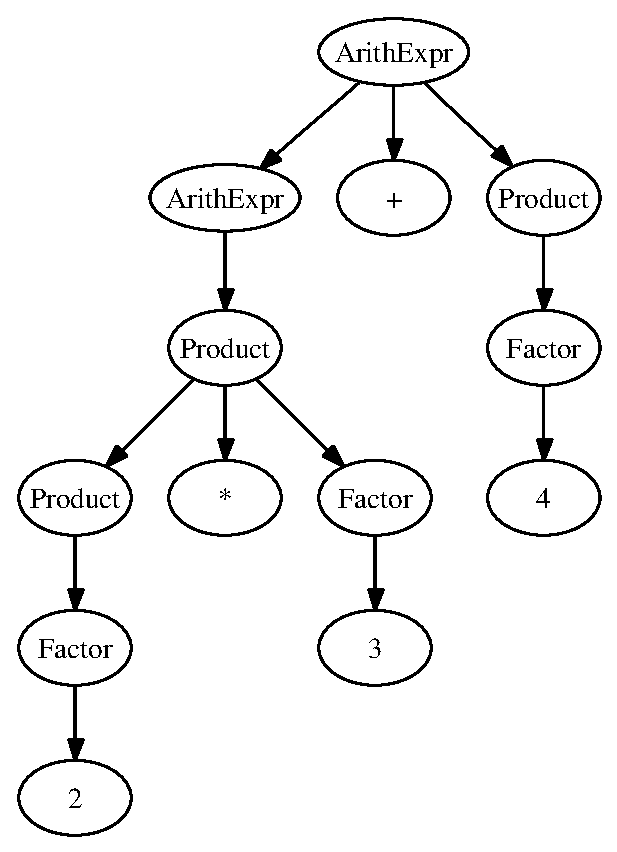
\epsfig{file=Abbildungen/parse-tree.eps, scale=0.7}
  \caption{Ein Parse-Baum f\"ur den String ``\texttt{2*3+4}''.}
  \label{fig:parse-tree.dot}
\end{figure}

Da B\"aume der in Abbildung \ref{fig:parse-tree.dot} gezeigten Art sehr schnell zu gro{\ss}
werden, vereinfachen wir diese B\"aume mit Hilfe der folgenden Regeln:
\begin{enumerate}
\item Ist $n$ ein innerer Knoten, der mit der Variablen $A$ beschriftet ist
      und gibt es unter den Kindern dieses Knotens genau ein Kind, dass mit einem Terminal $o$
      beschriftet ist,  so entfernen wir dieses Kind und beschriften den Knoten $n$ statt dessen mit dem
      Terminal $o$.
\item Hat ein innerer Knoten nur ein Kind, so ersetzen wir diesen Knoten durch sein Kind.
\end{enumerate}
Den Baum, den wir auf diese Weise erhalten, nennen wir den \emph{abstrakten Syntax-Baum}.
Abbildung \ref{fig:abstract-syntax-tree.dot} zeigt den abstrakten Syntax-Baum den wir
erhalten, wenn wir den in Abbildung \ref{fig:parse-tree.dot} gezeigten Parse-Baum nach
diesen Regeln vereinfachen.  Die in diesem Baum gespeicherte Struktur ist genau das, was
wir brauchen um den arithmetischen Ausdruck ``\texttt{2*3+4}'' auszuwerten, denn der Baum zeigt uns,
in welcher Reihenfolge die Operatoren ausgewertet werden m\"ussen.

\begin{figure}[!ht]
  \centering
      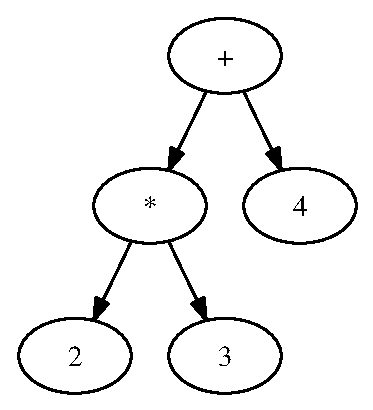
\epsfig{file=Abbildungen/abstract-syntax-tree.eps, scale=0.7}
  \caption{Ein abstrakter Syntax-Baum f\"ur den String ``\texttt{2*3+4}''.}
  \label{fig:abstract-syntax-tree.dot}
\end{figure}

\subsection{Mehrdeutige Grammatiken}
Die zu Anfang des Abschnitts \ref{kontextfreie} angegebene Grammatik zur Beschreibung arithmetischer
Ausdr\"ucke erscheint durch ihre Unterscheidung der syntaktischen Kategorien \textsl{arithExpr},
\textsl{product} und \textsl{factor} unn\"otig kompliziert.  Wir stellen eine einfachere Grammatik $G$
vor, welche dieselbe Sprache beschreibt:
\\[0.2cm]
\hspace*{1.3cm}
$G = \bigl\langle \{\textsl{expr}\}, \{ \textsc{Number}, \textsc{Variable}, \quoted{+}, \quoted{-}, \quoted{*}, \quoted{/}, \quoted{(}, \quoted{)} \}, R, \textsl{expr} \bigr\rangle$,
\\[0.2cm]
wobei die Regeln $R$ wie folgt gegeben sind:
\begin{eqnarray*}
  \textsl{expr} & \rightarrow & \textsl{expr} \quoted{+} \textsl{expr}  \\
                & \mid        & \textsl{expr} \quoted{-} \textsl{expr}  \\
                & \mid        & \textsl{expr} \quoted{*} \textsl{expr}  \\
                & \mid        & \textsl{expr} \quoted{/} \textsl{expr}  \\
                & \mid        & \quoted{(} \textsl{expr} \quoted{)}     \\
                & \mid        & \textsc{Number}                         \\
                & \mid        & \textsc{Variable}                         
\end{eqnarray*}
Um zu zeigen, dass der String ``\texttt{2*3+4}'' in der von dieser Sprache erzeugten
Grammatik liegt, geben wir die folgende Ableitung an:
\begin{eqnarray*}
\textsl{expr} & \Rightarrow & \textsl{expr} \quoted{+} \textsl{expr}                           \\
              & \Rightarrow & \textsl{expr} \quoted{*} \textsl{expr} \quoted{+} \textsl{expr}  \\
              & \Rightarrow & \texttt{2} \quoted{*} \textsl{expr} \quoted{+} \textsl{expr}     \\
              & \Rightarrow & \texttt{2} \quoted{*} \texttt{3} \quoted{+} \textsl{expr}        \\
              & \Rightarrow & \texttt{2} \quoted{*} \texttt{3} \quoted{+} \texttt{4}           
\end{eqnarray*}
Diese Ableitung entspricht dem abstrakten Syntax-Baum, der in Abbildung
\ref{fig:abstract-syntax-tree.dot}
gezeigt ist.  Es gibt aber noch eine andere Ableitung des Strings ``\texttt{2*3+4}'' mit dieser Grammatik:
\begin{eqnarray*}
\textsl{expr} & \Rightarrow & \textsl{expr} \quoted{*} \textsl{expr}                           \\
              & \Rightarrow & \textsl{expr} \quoted{*} \textsl{expr} \quoted{+} \textsl{expr}  \\
              & \Rightarrow & \texttt{2} \quoted{*} \textsl{expr} \quoted{+} \textsl{expr}     \\
              & \Rightarrow & \texttt{2} \quoted{*} \texttt{3} \quoted{+} \textsl{expr}        \\
              & \Rightarrow & \texttt{2} \quoted{*} \texttt{3} \quoted{+} \texttt{4}           
\end{eqnarray*}
Dieser Ableitung entspricht der abstrakte Syntax-Baum, der in Abbildung
\ref{fig:abstract-syntax-tree-prod.dot} gezeigt ist.
Bei dieser Ableitung wird der String ``\texttt{2*3+4}'' offenbar als Produkt aufgefasst,
was der Konvention widerspricht, dass der Operator ``\texttt{*}'' st\"arker bindet als der Operator
``\texttt{+}''.  W\"urden wir den String anhand des letzten Syntax-Baums auswerten, w\"urden wir
offenbar ein falsches Ergebnis bekommen! 
\begin{figure}[!ht]
  \centering
      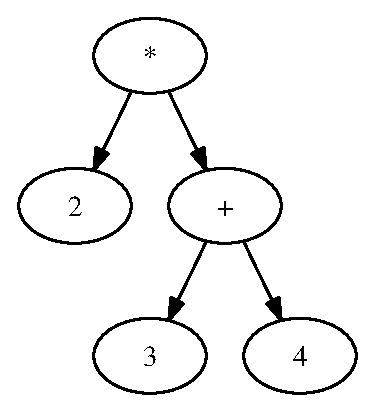
\epsfig{file=Abbildungen/abstract-syntax-tree-prod.eps, scale=0.6}
  \caption{Ein anderer abstrakter Syntax-Baum f\"ur den String ``\texttt{2*3+4}''.}
  \label{fig:abstract-syntax-tree-prod.dot}
\end{figure}
Die Ursache dieses Problems ist die Tatsache, dass die zuletzt angegebene Grammatik \underline{mehrdeuti}g ist.
Eine solche Grammatik ist zum Parsen ungeeignet.  Leider ist die Frage, ob eine gegebene
Grammatik mehrdeutig ist, im Allgemeinen nicht
\href{http://en.wikipedia.org/wiki/Ambiguous_grammar#Recognizing_ambiguous_grammars}{entscheidbar}:
Es l\"asst sich zeigen, dass diese Frage zum
\href{http://en.wikipedia.org/wiki/Post_correspondence_problem}{\emph{Postschen Korrespondenz-Problem}} 
\"aquivalent ist.  Da das Postsche Korrespondenz-Problem als unl\"osbar nachgewiesen wurde, ist auch die
Frage, ob eine Grammatik mehrdeutig ist, unl\"osbar.
Ein Beweis dieser Behauptungen findet sich beispielsweise in dem Buch von Hopcroft, Motwani und
Ullman \cite{hopcroft:06}. 


\example
Es sei $\Sigma = \{ \squoted{A}, \squoted{B} \}$.  Die Sprache $L$ enthalte alle die W\"orter
aus $\Sigma^*$, bei denen die Buchstaben \squoted{A} and \squoted{B} mit der gleichen
H\"aufigkeit auftreten, es gilt also
\\[0.2cm]
\hspace*{1.3cm}
$L = \bigl\{ w \in \Sigma^* \mid \textsl{count}(w, \squoted{A}) = \textsl{count}(w, \squoted{B}) \bigr\}$.
\\[0.2cm]
Dann wird die Sprache $L$ durch die kontextfreie Grammatik $G_1 = \langle \{s\}, \Sigma, R_1, s \rangle$ beschrieben,
deren Regeln wie folgt gegeben sind:
\\[0.2cm]
\hspace*{1.3cm}
$\textsl{s} \;\rightarrow\; \quoted{A} s \quoted{B} s \;\mid\; \quoted{B} s \quoted{A} s \;\mid\; \varepsilon$
\\[0.2cm]
Der Grund ist, dass ein String $w \in L$ entweder mit einem \squoted{A} oder mit einem \squoted{B}
beginnt.  Im ersten Fall muss es zu diesem \squoted{A} ein korrespondierendes \squoted{B} geben, denn
die Anzahl der Auftreten von \squoted{A} und \squoted{B} sind gleich.  Fassen wir den Buchstaben
\squoted{A} wie eine \"offnende Klammer auf und interpretieren den Buchstaben \squoted{B} als die zu
\squoted{A} korrespondierende schlie{\ss}ende Klammer, so ist klar, dass der String, der zwischen diesen
beiden Auftreten von \squoted{A} und \squoted{B} liegt, ebenfalls gleich viele Auftreten von
\squoted{A} wie von \squoted{B} hat.  Genauso muss dies dann f\"ur den Rest des Strings gelten, der nach
dem \squoted{B} folgt.  Diese \"Uberlegung erkl\"art die Regel
\\[0.2cm]
\hspace*{1.3cm}
$\textsl{s} \;\rightarrow\; \quoted{A} s \quoted{B} s$
\\[0.2cm]
Die Regel
\\[0.2cm]
\hspace*{1.3cm}
$\textsl{s} \;\rightarrow\; \quoted{B} s \quoted{A} s$
\\[0.2cm]
l\"asst sich in analoger Weise erkl\"aren,  wenn wir den Buchstaben \squoted{B} als \"offnende Klammer und
\squoted{A} als schlie{\ss}ende Klammer interpretieren. 

Diese Grammatik ist allerdings mehrdeutig: Betrachten wir beispielsweise den String 
``\texttt{abab}'', so stellen wir fest, dass sich dieser prinzipiell auf zwei Arten ableiten l\"asst:
\begin{eqnarray*}
  s & \Rightarrow &\quoted{A} s \quoted{B} s                       \\
    & \Rightarrow &\quoted{A} \quoted{B} s                         \\
    & \Rightarrow &\quoted{A} \quoted{B}\quoted{A} s \quoted{B} s \\
    & \Rightarrow &\quoted{A} \quoted{B}\quoted{A} \quoted{B} s   \\
    & \Rightarrow &\quoted{A} \quoted{B}\quoted{A} \quoted{B} 
\end{eqnarray*}
Eine andere Ableitung desselben Strings ergibt sich, wenn wir im zweiten Ableitungs-Schritt nicht das erste
$s$ durch $\varepsilon$ ersetzen sondern statt dessen das zweite $s$ durch $\varepsilon$ ersetzen:
\begin{eqnarray*}
  s & \Rightarrow &\quoted{A} s \quoted{B} s                       \\
    & \Rightarrow &\quoted{A} s \quoted{B}                         \\
    & \Rightarrow &\quoted{A} \quoted{B} s\quoted{A} s \quoted{B} \\
    & \Rightarrow &\quoted{A} \quoted{B}\quoted{A} s \quoted{B}   \\
    & \Rightarrow &\quoted{A} \quoted{B}\quoted{A} \quoted{B}     \\
\end{eqnarray*}
Abbildung \ref{fig:ambiguous-a.dot} zeigt die Parse-B\"aume, die sich aus den beiden Ableitungen ergeben.
Wir k\"onnen erkennen, dass die Struktur dieser B\"aume unterschiedlich ist:  Im ersten Fall geh\"ort das erste
``\texttt{A}'' zu dem ersten ``\texttt{B}'', im zweiten Fall geh\"ort das erste ``\texttt{A}'' zu dem letzten
``\texttt{B}''.

\begin{figure}[!ht]
      \epsfig{file=Abbildungen/ambiguous-a.eps, scale=0.6}
\quad
      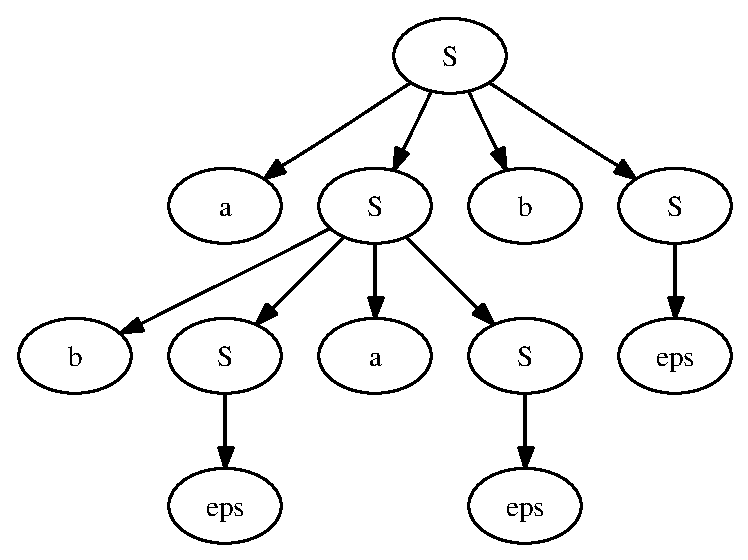
\epsfig{file=Abbildungen/ambiguous-b.eps, scale=0.6}
  \caption{Zwei strukturell verschiedene Parse-B\"aume f\"ur den String ``\texttt{ABAB}''.}
  \label{fig:ambiguous-a.dot}
\end{figure}

Wir definieren nun eine  kontextfreie Grammatik $G_2 = \langle \{s, u, v, x, y\}, \Sigma, R_2, s \rangle$,
deren Regeln wie folgt gegeben sind:
\hspace*{1.3cm}
\begin{eqnarray*}
\textsl{s} & \rightarrow & \textsl{u} \textsl{s} \;\mid\; \textsl{v} \textsl{s} \;\mid\; \varepsilon \\[0.2cm]
\textsl{u} & \rightarrow &\quoted{A} \textsl{x} \quoted{B}                \\[0.2cm]
\textsl{v} & \rightarrow & \quoted{B} \textsl{y} \quoted{A}                \\[0.2cm]
\textsl{x} & \rightarrow & \textsl{u} \textsl{x} \;\mid\; \varepsilon \\[0.2cm]
\textsl{y} & \rightarrow & \textsl{v} \textsl{y} \;\mid\; \varepsilon          
\end{eqnarray*}
Um die Sprachen, die von den einzelnen Variablen erzeugt werden, klarer beschreiben zu
k\"onnen, definieren wir f\"ur zwei Strings $\sigma$ und $\omega$ die Relation $\sigma \preceq \omega$ (lese: $\sigma$ ist ein
Pr\"afix von $\omega$) wie folgt:
\\[0.2cm]
\hspace*{1.3cm}
$\sigma \preceq \omega \quad \stackrel{\rm{def}}{\Longleftrightarrow} \exists \tau \in \Sigma^*: \sigma \tau = \omega$
\\[0.2cm]
Sodann bemerken wir, dass von den syntaktischen Variablen $x$ und $y$ die folgenden
Sprachen erzeugt werden:
\\[0.2cm]
\hspace*{1.3cm} 
$L(x) = \bigl\{ \omega \in \Sigma^* \mid \omega \in L \;\wedge\; \forall \sigma \preceq \omega : 
                  \textsl{count}(\sigma,\squoted{B}) \leq \textsl{count}(\sigma,\squoted{A}) \bigr\}$
\quad und \\[0.2cm]
\hspace*{1.3cm}
$L(y) = \bigl\{ \omega \in \Sigma^* \mid \omega \in L \;\wedge\; \forall \sigma \preceq \omega : 
                  \textsl{count}(\sigma, \squoted{A}) \leq \textsl{count}(\sigma, \squoted{B}) \bigr\}$.
\\[0.2cm]
Ist $w \in L(x)$, so gibt es zu jedem Auftreten des Buchstabens ``\texttt{B}'' in dem String $w$ ein
dazu korrespondierendes Auftreten des Buchstabens ``\texttt{A}'', das dem Auftreten des Buchstabens
``\texttt{B}'' vorangeht.  W\"urden wir den Buchstaben
``\texttt{A}'' durch eine \"offnende Klammer und den Buchstaben ``\texttt{B}'' durch eine schlie{\ss}ende
Klammer ersetzen, so wird also niemals eine Klammer geschlossen, die nicht vorher ge\"offnet wurde.
Damit ist klar, dass in einem String der Form
\\[0.2cm]
\hspace*{1.3cm}
``\texttt{A}'' $w$ ``\texttt{B}'' \quad mit $w \in L(x)$ 
\\[0.2cm]
das zu dem ersten ``\texttt{A}'' korrespondierende ``\texttt{B}'' nur das letzte ``\texttt{B}'' sein kann.
Analog k\"onnen wir sehen, dass in einem String der Form
\\[0.2cm]
\hspace*{1.3cm}
``\texttt{B}'' $w$ ``\texttt{A}'' \quad mit $w \in L(Y)$ 
\\[0.2cm]
das zu dem ersten ``\texttt{B}'' korrespondierende ``\texttt{A}'' nur das letzte ``\texttt{A}'' sein kann.

Ein String der Sprache $L$ f\"angt nun entweder mit ``\texttt{A}'' oder mit ``\texttt{B}''
an.  Im ersten Fall interpretieren wir das ``\texttt{A}'' als \"offnende Klammer und 
das ``\texttt{B}'' als schlie{\ss}ende Klammer und suchen nun das ``\texttt{B}'', das dem
``\texttt{A}'' am Anfang des Strings zugeordnet ist.  Der String, der mit dem
``\texttt{A}'' anf\"angt und dem ``\texttt{B}'' endet, liegt in der Sprache $L(u)$.
Auf dieses ``\texttt{B}'' kann dann noch ein weiterer Teilstring folgen, der
gleich viele ``\texttt{A}''s und ``\texttt{B}''s enth\"alt.  Ein solcher Teilstring liegt
offensichtlich ebenfalls in der Sprache $L$ und kann daher von $s$ mittels der Regel
\\[0.2cm]
\hspace*{1.3cm}
$\textsl{s} \rightarrow \textsl{u}\textsl{s}$
\\[0.2cm]
erzeugt werden.
Im zweiten Fall f\"angt der String mit einem ``\texttt{B}'' an.  Dieser Fall ist
analog zum ersten Fall.    \qed
\vspace*{0.3cm}

In dem obigen Beispiel hatten wir Gl\"uck und konnten eine Grammatik finden, mit der sich
die Sprache eindeutig parsen l\"asst.  Es  gibt allerdings auch kontextfreie Sprachen, die 
\href{http://en.wikipedia.org/wiki/Ambiguous_grammar#Inherently_ambiguous_languages}{inh\"arent mehrdeutig}
sind: Es l\"asst sich beispielsweise zeigen, dass f\"ur das Alphabet 
$\Sigma =  \{ \squoted{A}, \squoted{B}, \squoted{C}, \squoted{D} \}$
die Sprache
\\[0.2cm]
\hspace*{1.3cm}
$L =  \bigl\{ \mathtt{A}^m \mathtt{B}^m \mathtt{C}^n \mathtt{D}^n \mid m, n \in \mathbb{N} \bigr\}
 \cup \bigl\{ \mathtt{A}^m \mathtt{B}^n \mathtt{C}^n \mathtt{D}^m \mid m, n \in \mathbb{N} \bigr\}
$
\\[0.2cm]
kontextfrei ist, aber jede Grammatik $G$ mit der Eigenschaft $L = L(G)$ ist
notwendigerweise mehrdeutig.  Das Problem ist, dass f\"ur gewisse gro{\ss}e Zahlen $n\in \mathbb{N}$ ein
String der Form 
\\[0.2cm]
\hspace*{1.3cm}
$\mathtt{A}^n \mathtt{B}^n \mathtt{C}^n \mathtt{D}^n$
\\[0.2cm]
immer zwei strukturell verschiedene Parse-B\"aume besitzen muss.  Ein Beweis dieser Behaupung
findet sich in der ersten Auflage des Buchs von  Hopcroft und Ullman auf Seite 100 \cite{hopcroft:79}.   

\section{Top-Down-Parser}
In diesem Abschnitt stellen wir ein Verfahren vor, mit dem sich eine ganze Reihe von
Grammatiken bequem parsen lassen.  Die Grundidee ist einfach:  Um einen String $w$ mit
Hilfe einer Grammatik-Regel der Form
\\[0.2cm]
\hspace*{1.3cm}
$\textsl{a} \rightarrow \textsl{X}_1 \textsl{X}_2 \cdots \textsl{X}_n$
\\[0.2cm]
zu parsen, versuchen wir, zun\"achst ein $X_1$ zu parsen.  Dabei zerlegen wir den String $w$ in die
Form
$w = w_1 r_1$ so, dass $w_1 \in L(X_1)$ gilt.  Dann versuchen wir, in dem Rest-String
$r_1$ ein $X_2$ zu parsen und zerlegen dabei $r_1$ so, dass $r_1 = w_2 r_2$ mit 
$w_2 \in L(X_2)$ gilt.  Setzen wir diesen Prozess fort, so haben wir zum Schluss den String $w$ in
\\[0.2cm]
\hspace*{1.3cm}
$w = w_1 w_2 \cdots w_n$ \quad mit $w_i \in L(X_i)$ f\"ur alle $i=1,\cdots,n$
\\[0.2cm]
aufgespaltet.  Leider funktioniert dieses Verfahren dann nicht, wenn die Grammatik
\emph{links-rekursiv} ist, dass hei{\ss}t, dass eine Regel die Form
\\[0.2cm]
\hspace*{1.3cm}
$\textsl{a} \rightarrow \textsl{a} \beta$
\\[0.2cm]
hat, denn dann w\"urden wir um ein $\textsl{a}$ zu parsen sofort wieder rekursiv versuchen, 
ein $a$ zu parsen und w\"aren damit in einer Endlos-Schleife.  Es gibt mehrere M\"oglichkeiten, um mit
diesem Problem umzugehen:
\begin{enumerate}
\item Wir k\"onnen die Grammatik so umschreiben, dass sie danach nicht mehr links-rekursiv
      ist.
\item Wir k\"onnen versuchen, den String \emph{r\"uckw\"arts} zu parsen, d.h.~bei einer
      Regel der Form
      \\[0.2cm]
      \hspace*{1.3cm}
      $\textsl{a} \rightarrow \textsl{X}_1 \textsl{X}_2 \cdots \textsl{X}_n$
      \\[0.2cm]
      versuchen wir als erstes, ein $X_n$ am Ende eines zu parsenden Strings $w$ zu
      entdecken und arbeiten dann den String $w$ von hinten  nach vorne ab.  
\item Die einfachste L\"osung erhalten wir, wenn wir uns klar machen, dass kontextfreie
      Grammatiken nicht unbedingt die bequemste Art darstellen, eine Sprache 
      zu beschreiben.  Wir werden daher den Begriff der \emph{erweiterten Backus-Naur-Form}-Grammatik
      (abgek\"urzt \textsc{Ebnf}-Grammatik) einf\"uhren.  Hierbei handelt es sich um eine Verallgemeinerung des
      Begriffs der kontextfreien Grammatik.  Theoretisch ist die Ausdrucksst\"arke der
      \textsc{Ebnf}-Grammatiken dieselbe wie die Ausdrucksst\"arke der kontextfreien Grammatiken.
      In der Praxis zeigt sich aber, dass die Konstruktion von Top-Down-Parsern f\"ur
      \textsc{Ebnf}-Grammatiken einfacher ist, weil dort die Links-Rekursion durch eine Iteration ersetzt
      werden kann.
\end{enumerate}
Im Rahmen dieses Kapitels werden wir alle oben genannten Verfahren anhand der Grammatik f\"ur
arithmetische Ausdr\"ucke ausf\"uhrlich diskutieren.  

\subsection{Umschreiben der Grammatik$^*$ \label{links-rekursion}}
In der folgenden Grammatik ist $a$ eine syntaktische Variable und die griechischen Buchstaben $\beta$ und
$\gamma$ stehen f\"ur irgendwelche Strings, die aus syntaktischen Variablen und Tokens bestehen.
Wird die syntaktische Variable $a$ durch die beiden Regeln
\\[0.2cm]
\hspace*{1.3cm}
$
\begin{array}[t]{lcl}
a & \rightarrow & a \beta \\
  & \mid        & \gamma
\end{array}
$
\\[0.2cm]
definiert, so hat eine Ableitung von $a$, bei der zun\"achst immer die syntaktische Variable $a$ ersetzt
wird, die Form 
\\[0.2cm]
\hspace*{1.3cm}
$a \Rightarrow a \beta \Rightarrow a \beta \beta \Rightarrow a \beta \beta \beta
 \Rightarrow \cdots \Rightarrow a \beta^n \Rightarrow \gamma \beta^n$.
\\[0.2cm]
Damit sehen wir, dass die durch die syntaktische Variable $a$ beschriebene Sprache $L(a)$ aus allen den
Strings besteht, die sich aus dem Ausdruck $\gamma \beta^n$ ableiten lassen:
\\[0.2cm]
\hspace*{1.3cm}
$L(a) = \bigl\{ w \in \Sigma^* \mid \exists n \in \mathbb{N}_0: \gamma \beta^n \Rightarrow^* w \bigr\}$.
\\[0.2cm]
Diese Sprache kann offenbar auch durch die folgenden Regeln f\"ur $a$ beschrieben werden:
\\[0.2cm]
\hspace*{1.3cm}
$
\begin{array}[t]{lcl}
a & \rightarrow & \gamma b \\[0.2cm]
b & \rightarrow & \beta b  \\
  & \mid        & \varepsilon 
\end{array}
$
\\[0.2cm]
Hier haben wir die Hilfs-Variable $b$ eingef\"uhrt.  Die Ableitungen, die von dem Nicht-Terminal $b$
ausgehen, haben die Form
\\[0.2cm]
\hspace*{1.3cm} $b \Rightarrow \beta b \Rightarrow \beta \beta b \Rightarrow \cdots \Rightarrow
\beta^n b \Rightarrow \beta^n$.
\\[0.2cm]
Folglich beschreibt das Nicht-Terminal $b$ die Sprache
\\[0.2cm]
\hspace*{1.3cm} $L(b) = \bigl\{ w \in \Sigma \mid \exists n \in \mathbb{N}_0: \beta^n \Rightarrow w
\bigr\}$.
\\[0.2cm]
Damit ist klar, dass auch mit der oben angegeben Grammatik
\\[0.2cm]
\hspace*{1.3cm} $L(a) = \bigl\{ w \in \Sigma^* \mid \exists n \in \mathbb{N}_0: \gamma \beta^n
\Rightarrow^* w \bigr\}$
\\[0.2cm]
gilt.  Um die Links-Rekursion aus der in Abbildung \ref{fig:Expr} auf Seite \pageref{fig:Expr}
gezeigten Grammatik zu entfernen, m\"ussen wir das obige Beispiel verallgemeinern.  Wir betrachten
jetzt den allgemeinen Fall und nehmen an, dass ein Nicht-Terminal $a$ durch Regeln der Form
\\[0.2cm]
\hspace*{1.3cm} $
\begin{array}[t]{lcl}
a & \rightarrow & a \beta_1 \\
  & \mid        & a \beta_2 \\
  & \vdots      & \vdots    \\
  & \mid        & a \beta_k \\[0.2cm]
  & \mid        & \gamma_1  \\
  & \vdots      & \vdots    \\
  & \mid        & \gamma_l
\end{array}
$
\\[0.2cm]
beschrieben wird.  Wir k\"onnen diesen Fall durch Einf\"uhrung zweier Hilfs-Variablen $b$ und $c$ auf
den ersten Fall zur\"uckf\"uhren:
\\[0.2cm]
\hspace*{1.3cm}
$
\begin{array}[t]{lcl}
a & \rightarrow & a b \mid c                         \\[0.2cm]
b & \rightarrow & \beta_1 \mid \cdots \mid \beta_k   \\[0.2cm]
c & \rightarrow & \gamma_1 \mid \cdots \mid \gamma_l
\end{array}
$
\\[0.2cm]
Dann k\"onnen wir die Grammatik umschreiben, indem wir eine neue Hilfs-Variable, nennen wir sie $l$
f\"ur Liste, einf\"uhren und erhalten
\\[0.2cm]
\hspace*{1.3cm}
$
\begin{array}[t]{lcl}
a & \rightarrow & c\;l                   \\[0.2cm]
l & \rightarrow & b\;l \mid \varepsilon.  
\end{array}
$
\\[0.2cm]
Die Hilfs-Variablen $b$ und $c$ k\"onnen nun wieder eliminiert werden und dann bekommen wir die folgende
Grammatik: 
\\[0.2cm]
\hspace*{1.3cm}
$
\begin{array}[t]{lcl}
a & \rightarrow & \gamma_1\;l \;\mid\; \gamma_2\;l \;\mid\; \cdots \;\mid\; \gamma_l\;l  \\[0.2cm]
l & \rightarrow & \beta_1 \;l \;\mid\; \beta_2 \;l \;\mid\; \cdots \;\mid\; \beta_k \;l \;\mid\; \varepsilon
\end{array}
$
\begin{figure}[htbp]
  \begin{center}    
  \framebox{
  \framebox{
  \begin{minipage}[t]{8cm}
  \begin{eqnarray*}
  \textsl{expr}    & \rightarrow & \;\textsl{expr} \quoted{+} \textsl{product}  \\
                   & \mid        & \;\textsl{expr} \quoted{-} \textsl{product}  \\
                   & \mid        & \;\textsl{product}                           \\[0.2cm]
  \textsl{product} & \rightarrow & \;\textsl{product} \quoted{*} \textsl{factor}\\
                   & \mid        & \;\textsl{product} \quoted{/} \textsl{factor}\\
                   & \mid        & \;\textsl{factor}                            \\[0.2cm]
  \textsl{factor}  & \rightarrow &   \quoted{(} \textsl{expr} \quoted{)}        \\
                   & \mid        & \;\textsc{Number} 
  \end{eqnarray*}
  \vspace*{-0.5cm}
  \end{minipage}}}
  \end{center}
  \caption{Links-rekursive Grammatik f\"ur arithmetische Ausdr\"ucke.}
  \label{fig:Expr}
\end{figure}
\vspace*{0.3cm}

\noindent
Wenden wir dieses Verfahren auf die in Abbildung \ref{fig:Expr} gezeigte Grammatik f\"ur arithmetische
Ausdr\"ucke an, so erhalten wir die in Abbildung \ref{fig:Expr2} gezeigte Grammatik.

\begin{figure}[htbp]
  \begin{center}    
  \framebox{
  \framebox{
  \begin{minipage}[t]{9cm}
  \begin{eqnarray*}
  \textsl{expr}        & \rightarrow & \;\textsl{product}\;\;\textsl{exprRest}            \\[0.2cm]
  \textsl{exprRest}    & \rightarrow & \quoted{+} \textsl{product}\;\;\textsl{exprRest}   \\
                       & \mid        & \quoted{-} \textsl{product}\;\;\textsl{exprRest}   \\
                       & \mid        & \;\varepsilon                                      \\[0.2cm]
  \textsl{product}     & \rightarrow & \;\textsl{factor}\;\;\textsl{productRest}          \\[0.2cm]
  \textsl{productRest} & \rightarrow & \quoted{*} \textsl{factor}\;\;\textsl{productRest} \\
                       & \mid        & \quoted{/} \textsl{factor}\;\;\textsl{productRest} \\
                       & \mid        & \;\varepsilon                                      \\[0.2cm]
  \textsl{factor}      & \rightarrow & \quoted{(} \textsl{expr} \quoted{)}                \\
                       & \mid        & \;\textsc{Number} 
  \end{eqnarray*}
  \vspace*{-0.5cm}
  \end{minipage}}}
  \end{center}
  \caption{Grammatik f\"ur arithmetische Ausdr\"ucke ohne Links-Rekursion.}
  \label{fig:Expr2}
\end{figure}

\noindent
Die Variablen \textsl{exprRest} und \textsl{productRest} k\"onnen wie folgt interpretiert werden:
\begin{enumerate}
\item \textsl{exprRest} beschreibt eine Liste der Form
      \\[0.2cm]
      \hspace*{1.3cm}
      $\textsl{op} \;\textsl{product} \;\cdots \;\textsl{op}\; \textsl{product}$,
      \\[0.2cm]
      wobei $\textsl{op} \in \{ \quoted{+}, \quoted{-} \}$ gilt.
\item \textsl{productRest} beschreibt eine Liste der Form
      \\[0.2cm]
      \hspace*{1.3cm}
      $\textsl{op} \;\textsl{factor} \;\cdots \;\textsl{op} \;\textsl{factor}$,
      \\[0.2cm]
      wobei $\textsl{op} \in \{ \quoted{*}, \quoted{/} \}$ gilt. 
\end{enumerate}


\exercise
\begin{enumerate}
\item[(a)] Die folgende Grammatik beschreibt regul\"are Ausdr\"ucke:
      \begin{center}    
          \framebox{
            \begin{minipage}[t]{9cm}
              \begin{eqnarray*}
                \textsl{regExp} & \rightarrow & \;\textsl{regExp} \quoted{+} \textsl{regExp}    \\
                                & \mid        & \;\textsl{regExp} \;\;\textsl{regExp}           \\
                                & \mid        & \;\textsl{regExp}\quoted{*}                     \\
                                & \mid        & \quoted{(} \textsl{regExp} \quoted{)}           \\
                                & \mid        & \;\textsc{Letter}                               
              \end{eqnarray*}
              \vspace*{-0.5cm}
            \end{minipage}}
      \end{center}
      Diese Grammatik verwendet nur die  syntaktische Variable $\{ \textsl{regExp} \}$ und die folgenden 
      Terminale
      \\[0.2cm]
      \hspace*{1.3cm}
      \squoted{+}, \squoted{*}, \squoted{(}, \squoted{)}, \textsc{Letter}.
      \\[0.2cm]
      Da die Grammatik mehrdeutig ist, ist diese Grammatik zum Parsen ungeeignet.
      Transformieren Sie diese Grammatik in eine eindeutige Grammatik, bei welcher der
      Postfix-Operator ``\texttt{*}'' st\"arker bindet als die Konkatenation zweier regul\"arer
      Ausdr\"ucke, w\"ahrend der Operator ``\texttt{+}'' schw\"acher bindet als die Konkatenation. 
      Orientieren Sie sich dabei an der Grammatik f\"ur arithmetische Ausdr\"ucke und f\"uhren
      Sie geeignete neue syntaktische Variablen ein.
\item[(b)] Entfernen Sie die Links-Rekursion aus der in Teil (a) dieser Aufgabe erstellten
      Grammatik. \eox
\end{enumerate}

\begin{figure}[htbp]
  \begin{center}    
  \framebox{
  \framebox{
  \begin{minipage}[t]{9cm}
  \begin{eqnarray*}
  \textsl{s}  & \rightarrow & \textsl{a} \quoted{X}  \\
              & \mid        & \squoted{Y}            \\[0.2cm]
  \textsl{a}  & \rightarrow & \textsl{b} \quoted{Y}  \\
              & \mid        & \quoted{x}             \\[0.2cm]
  \textsl{b}  & \rightarrow & \textsl{s} \quoted{Z}  
  \end{eqnarray*}
  \vspace*{-0.5cm}
  \end{minipage}}}
  \end{center}
  \caption{Wechselseitige Links-Rekursion.}
  \label{fig:mutual-left-recursion}
\end{figure}

Bei den bisher diskutierten Beispielen war die Links-Rekursion der Grammatik unmittelbar anzusehen.
Es gibt allerdings F\"alle, in denen die Links-Rekursion ihren Ursprung in 
\emph{wechselseitiger Rekursion} hat.
Abbildung \ref{fig:mutual-left-recursion} auf Seite \pageref{fig:mutual-left-recursion} zeigt ein
solches Beispiel: Bei der dort angegebenen Grammatik erstreckt sich die Links-Rekursion \"uber drei Stufen:
Ein $s$ kann mit einem $a$ beginnen, das mit einem $b$ beginnen kann, welches dann wieder mit einem
$s$ beginnt.  Eine Links-Rekursion der Form
\\[0.2cm]
\hspace*{1.3cm}
$a \rightarrow a \beta$
\\[0.2cm]
bezeichnen wir als \emph{unmittelbare Links-Rekursion},  jede kompliziertere Form der
Links-Rekursion wird als \emph{allgemeine Links-Rekursion} bezeichnet.
Um allgemeine Links-Rekursion zu eliminieren, gehen wir wie folgt vor:
\begin{enumerate}
\item Zun\"achst nummerieren wir die syntaktischen Variablen der Grammatik in willk\"urlicher Weise durch.
      Im Folgenden seien die Variablen mit $a_1$, $\cdots$, $a_n$ bezeichnet.  Durch diese
      Nummerierung wird implizit eine Ordnung $\succ$ auf den syntaktischen Variablen
      definiert, wir setzen
      \\[0.2cm]
      \hspace*{1.3cm}
      $a_1 \succ a_2 \succ \cdots \succ a_i \succ a_{i+1} \succ \cdots \succ a_n$.
\item Das Ziel ist nun, die Grammatik so umzuschreiben, dass f\"ur jede
      Grammatik-Regel der Form
      \\[0.2cm]
      \hspace*{1.3cm}
      $a \rightarrow b \gamma$ \quad die Ungleichung \quad $a \succ b$
      \\[0.2cm]
      gilt.  Dieses Ziel wird durch den folgenden Algorithmus erreicht:
      \\[0.2cm]
      \hspace*{1.3cm}
      \texttt{for (i = 1; i <= n; ++i) \{}  \\[0.1cm]
      \hspace*{1.8cm}
      \texttt{for (j = 1; j < i; ++j) \{} \\[0.1cm]
      \hspace*{2.3cm}
      \texttt{forall $(a_i \rightarrow a_j\gamma) \in R$ \{} \\[0.1cm]
      \hspace*{2.8cm}
      \texttt{let $a_j \rightarrow \delta_1 \;|\; \cdots \;|\; \delta_k$ be all $a_j$-productions } \\[0.1cm]
      \hspace*{2.8cm}
      \texttt{replace $a_i \rightarrow a_j\gamma$ by $a_i \rightarrow \delta_1 \gamma \;|\;\cdots\;|\;\delta_k \gamma$} \\[0.1cm]
      \hspace*{2.3cm} 
      \texttt{\}}  \\[0.1cm]
      \hspace*{1.8cm} 
      \texttt{\}}  \\[0.1cm]
      \hspace*{1.8cm} 
      \texttt{eliminate immediate left recursion for variable $a_i$}  \\
      \hspace*{1.3cm} 
      \texttt{\}}  
\end{enumerate}
Um den Algorithmus zu verstehen, f\"uhren wir zun\"achst einen neuen Begriff ein:  Falls die Grammatik
eine Regel der Form
\\[0.2cm]
\hspace*{1.3cm}
$a \rightarrow b \gamma$
\\[0.2cm]
enth\"alt, wobei $b$ eine syntaktische Variable ist, dann sagen wir, dass $a$ unmittelbar von $b$
abh\"angt.  Die Idee bei dem oben angegebenen Algorithmus ist nun, dass nach dem $i$-ten
Durchlaufen der \"au{\ss}eren \texttt{for}-Schleife die Variablen $a_1$, $\cdots$, $a_i$ nur noch unmittelbar
von solchen Variablen abh\"angen, die in der Aufz\"ahlung $a_1$, $\cdots$, $a_n$ auf diese  Variablen
folgen.  Formal gilt nach dem $i$-ten Durchlauf der \"au{\ss}eren \texttt{for}-Schleife f\"ur alle Indizes 
$k \in \{ 1, \cdots, i \}$:  Falls die Grammatik eine Regel der Form
\\[0.2cm]
\hspace*{1.3cm}
$a_k \rightarrow a_l \beta$ 
\\[0.2cm]
enth\"alt, dann muss $l > k$ gelten.  Es ist leicht zu sehen, dass diese Invariante tats\"achlich gilt:
Vor dem $i$-ten Durchlauf gilt die Invariante f\"ur die Indizes der Menge $\{1, \cdots, i-1\}$.  Die
Variable $a_i$ selber kann dann noch unmittelbar von den Variablen $a_1$, $\cdots$, $a_n$ abh\"angen.
In der inneren \texttt{for}-Schleife erreichen wir, dass nacheinander die unmittelbaren
Abh\"angigkeiten von $a_1$, $\cdots$, $a_{i-1}$ aufgel\"ost werden.  Anschlie{\ss}end kann $a_i$ h\"ochstens
noch unmittelbar von $a_i$ abh\"angen.  Um diese Abh\"angigkeit gegebenenfalls aufzul\"osen, f\"uhren wir
die bereits fr\"uher diskutierte Transformation zur Elimination unmittelbarer Links-Rekursion durch.
Anschlie{\ss}end h\"angt $a_i$ h\"ochstens noch 
unmittelbar von $a_{i+1}$, $\cdots$, $a_n$ ab.  L\"auft die Schleife bis zum Ende durch, ist damit
die Links-Rekursion vollst\"andig eliminiert, denn dann kann jede Variable nur von solchen
Variablen abh\"angen, die in der Aufz\"ahlung $a_1$ $\cdots$, $a_n$ hinter ihr stehen.  Folglich ist 
kein Zyklus der Form 
\\[0.2cm]
\hspace*{1.3cm}
$a_i \Rightarrow a_j\beta \Rightarrow \cdots \Rightarrow a_i\gamma$
\\[0.2cm]
mehr m\"oglich.

\example
Wir demonstrieren das Verfahren an der in Abbildung \ref{fig:mutual-left-recursion} gezeigten
Grammatik.  Dazu ordnen wir zun\"achst die Variablen in der Form
\\[0.2cm]
\hspace*{1.3cm}
$s, a, b$
\\[0.2cm]
an, mit der Notation des oben angegebenen Algorithmus gilt also $a_1 := s$, $a_2 := a$ und 
$a_3 := b$.
\begin{enumerate}
\item $i = 1$:  Da $\{1, \cdots, i-1 \} = \{\}$ gilt,  wird in diesem Fall die innere
      \texttt{for}-Schleife nicht ausgef\"uhrt.  Wir m\"ussen lediglich
      die unmittelbare Links-Rekursion in der Variablen $s$ entfernen.  Da die Grammatik aber f\"ur
      $s$ keine unmittelbare Links-Rekursion enth\"alt, ist in diesem Fall nichts zu tun.
\item $i = 2$:  In diesem Schritt m\"ussen wir in der inneren \texttt{for}-Schleife sicherstellen,
      dass $a$ nicht unmittelbar von $s$ abh\"angt.  da $a$ in der gegebenen Grammatik nicht
      unmittelbar von $s$ abh\"angt, ist bei der inneren \texttt{for}-Schleife wieder nichts zu tun.

      Weiter m\"ussen wir die unmittelbare Rekursion aus allen Regeln f\"ur $a$ eliminieren.  Da 
      es f\"ur die Variable $a$ keine unmittelbare Rekursion gibt, ist an dieser Stelle ebenfalls nichts
      zu tun.
\item $i = 3$:  In diesem Fall kommen f\"ur die innere \texttt{for}-Schleife zwei Werte von $j$
      in Frage, die wir nacheinander behandeln m\"ussen:
      \begin{enumerate}
      \item $j = 1$:  Hier m\"ussen wir sicherstellen, dass $b$ nicht unmittelbar von $s$ abh\"angt.
            Bei der Regel
            \\[0.2cm]
            \hspace*{1.3cm}
            $b \rightarrow s \quoted{Z}$
            \\[0.2cm]
            ist dies aber der Fall.  Wir ersetzen daher das $s$ auf der rechten Seite dieser Regel
            durch die beiden rechten Seiten der Regeln f\"ur $s$ und erhalten f\"ur $b$ nun die Regeln
            \\[0.2cm]
            \hspace*{1.3cm}
            $b \rightarrow a \quoted{X} \squoted{Z}$ \quad und \quad
            $b \rightarrow \quoted{Y} \squoted{Z}$.
      \item $j = 2$:  Nun m\"ussen wir sicherstellen, dass $b$ nicht unmittelbar von $a$ abh\"angt.
            Bei der Regel
            \\[0.2cm]
            \hspace*{1.3cm}
            $b \rightarrow a \quoted{X} \squoted{Z}$ 
            \\[0.2cm]
            ist dies aber der Fall.  Wir ersetzen daher das $a$ auf der rechten Seite dieser Regel
            durch die beiden rechten Seiten der Regeln f\"ur $a$ und erhalten f\"ur $b$ nun insgesamt
            die folgenden Regeln:
            \\[0.2cm]
            \hspace*{1.3cm}
            $b \rightarrow b \quoted{Y} \squoted{X}\; \squoted{Z}$, \quad 
            $b \rightarrow \quoted{X} \squoted{X}\; \squoted{Z}$ \quad und \quad
            $b \rightarrow \quoted{Y} \squoted{Z}$.
      \end{enumerate}
      Diese Regeln enthalten nun nur noch ummittelbare Links-Rekursion, die wir mit dem fr\"uher
      beschriebenen Verfahren eliminieren.  Wir erhalten dann f\"ur $b$ die Regeln
      \\[0.2cm]
      \hspace*{1.3cm}
      $b \rightarrow \quoted{X} \squoted{X} \; \squoted{Z}\; l$ \quad und \quad
      $b \rightarrow \squoted{Y} \quoted{Z} l$,
      \\[0.2cm]
      wobei die neu eingef\"uhrte Variable $l$ durch die Regeln
      \\[0.2cm]
      \hspace*{1.3cm}
      $l \rightarrow \quoted{Y} \squoted{X}\; \squoted{Z}\; l$ \quad und \quad 
      $l \rightarrow \varepsilon$
      \\[0.2cm]
      definiert ist.
\end{enumerate}
Abbildung \ref{fig:mutual-left-recursion-2} zeigt die resultierende Grammatik.


\begin{figure}[htbp]
  \begin{center}    
  \framebox{
  \framebox{
  \begin{minipage}[t]{9cm}
  \begin{eqnarray*}
  \textsl{s}  & \rightarrow & \textsl{a} \quoted{X}  \\
              & \mid        & \squoted{Y}            \\[0.2cm]
  \textsl{a}  & \rightarrow & \textsl{b} \quoted{Y}  \\
              & \mid        & \squoted{X}             \\[0.2cm]
  \textsl{b}  & \rightarrow & \squoted{X} \quoted{X} \squoted{Z}\; \textsl{l} \\
              & \mid        & \squoted{Y} \quoted{Z} \textsl{l}               \\[0.2cm]
  \textsl{l}  & \rightarrow & \squoted{Y} \quoted{X} \squoted{Z}\; \textsl{l} \\
              & \mid        & \varepsilon      
  \end{eqnarray*}
  \vspace*{-0.5cm}
  \end{minipage}}}
  \end{center}
  \caption{Grammatik ohne Links-Rekursion.}
  \label{fig:mutual-left-recursion-2}
\end{figure}

Das letzte Beispiel zeigt, dass sich eine Grammatik durch die Elimination indirekter Links-Rekursion
stark aufbl\"ahen kann.  Zwar sind viele Grammatiken links-rekursiv, aber in der Regel
handelt es sich dabei um direkte Links-Rekursion.  Wechselseitige Links-Rekursion ist in den
Grammatiken, die Ihnen in der Praxis begegnen werden, ein eher seltenes Ph\"anomen.


\subsection{Implementing a Top Down Parser in \textsc{SetlX}}


\begin{figure}[!ht]
\centering
\begin{Verbatim}[ frame         = lines, 
                  framesep      = 0.3cm, 
                  firstnumber   = 1,
                  labelposition = bottomline,
                  numbers       = left,
                  numbersep     = -0.2cm,
                  xleftmargin   = 0.0cm,
                  xrightmargin  = 0.0cm,
                ]
    myParse := procedure(s) {
         [result, rl] := parseExpr(tokenizeString(s));
         assert(rl == [], "Parse Error: could not parse $tl$");
         return result;
    };
    parseExpr := procedure(tl) {
        [product, rl] := parseProduct(tl);
        return parseExprRest(product, rl);
    };
    parseExprRest := procedure(sum, tl) {
        match (tl) {
            case ["+" | rl] : [product, ql] := parseProduct(rl);
                              return parseExprRest(sum + product, ql);
            case ["-" | rl] : [product, ql] := parseProduct(rl);
                              return parseExprRest(sum - product, ql);
            default:          return [sum, tl];
        }
    };
    parseProduct := procedure(tl) {
        [factor, rl] := parseFactor(tl);
        return parseProductRest(factor, rl);
    };
    parseProductRest := procedure(product, tl) {
        match (tl) {
            case ["*" | rl] : [factor, ql] := parseFactor(rl);
                              return parseProductRest(product * factor, ql);
            case ["/" | rl] : [factor, ql] := parseFactor(rl);
                              return parseProductRest(product / factor, ql);
            default:          return [product, tl];
        }
    };
    parseFactor := procedure(tl) {
        match (tl) {
            case ["(" | rl] : [expr, ql] := parseExpr(rl);
                              assert(ql[1] == ")", "Parse Error");
                              return [expr, ql[2..]];
            default : return [tl[1], tl[2..]];
        }
    };
    tokenizeString := procedure(s) {
        tokenList := [];
        scan (s) {
            regex '0|[1-9][0-9]*' as [ number   ]: tokenList += [ int(number) ];
            regex '[-+*/()]'      as [ operator ]: tokenList += [ operator    ];
            regex '[ \t\v\n]+'                   : // skip
        }
        return tokenList;
    };
\end{Verbatim}
\vspace*{-0.3cm}
\caption{A top down parser for arithmetic expressions.}
\label{fig:rd-parser.stlx}
\end{figure}

\noindent
Now we are ready to implement a parser for recognizing arithmetic expressions.
Figure \ref{fig:rd-parser.stlx} on page
\pageref{fig:rd-parser.stlx} shows an implementation of a recursive decent parser in
\textsc{SetlX}. 
\begin{enumerate}
\item The main function is \texttt{myParse}\footnote{
            We had to name the function \texttt{myParse} instead of \texttt{parse} as 
            \textsc{SetlX} already implements a function with the name \texttt{parse}.
            This function parses strings as \textsc{SetlX} expressions.  The function
            \texttt{parse} returns a term representing the abstract syntax tree
            corresponding to the parsed expression.
      }.  This function takes a string $s$
      representing an arithmetic expression.  This string is tokenized using the 
      function \texttt{tokenizeString}.  The function \texttt{tokenizeString} turns a
      string into a list of tokens.  For example, the expression
      \\[0.2cm]
      \hspace*{1.3cm}
      \verb|tokenizeString("(1 + 2) * 3");|
      \\[0.2cm]
      returns the result
      \\[0.2cm]
      \hspace*{1.3cm}
      \verb|["(", 1, "+", 2, ")", "*", 3]|.
      \\[0.2cm]
      This list of tokens is then parsed by the function \texttt{parseExpr}.
      That function returns a pair: 
      \begin{enumerate}
      \item The first  component is the value of the arithmetic expression.
      \item The second component is the list of those tokens that have not been consumed
            when parsing the expression.  Of course, on a successful parse this list
            should be empty.
      \end{enumerate}
\item The function \texttt{parseExpr} implements the grammar rule
      \\[0.2cm]
      \hspace*{1.3cm}
      $\textsl{expr} \;\rightarrow\;\textsl{product}\;\;\textsl{exprRest}$. 
      \\[0.2cm]
      It takes a token list \texttt{tl} as input.  It will return a pair of the form
      \\[0.2cm]
      \hspace*{1.3cm}
      \texttt{[$v$, rl]},
      \\[0.2cm]
      where $v$ is the value of the arithmetic expression that has been parsed, while
      \texttt{rl} is the list of the remaining tokens.  For example, the expression
      \\[0.2cm]
      \hspace*{1.3cm}
      \verb|parseExpr(["(", 1, "+", 2, ")", "*", 3, ")", "*", 2])|
      \\[0.2cm]
      returns the result
      \\[0.2cm]
      \hspace*{1.3cm}
      \verb|[9, [")", "*", 2]]|.
      \\[0.2cm]
      Here, the part \verb|["(", 1, "+", 2, ")", "*", 3]| has been parsed and evaluated as
      the number $9$ and \verb|[")", "*", 2]| is the list of tokens that have not yet been
      processed.

      In order to parse an arithmetic expression, the function first parses a
      \textsl{product} and then it tries to parse the remaining tokens as an
      \textsl{exprRest}.   The function \texttt{parseExprRest} that is used to parse an
      \textsl{exprRest} needs two arguments:
      \begin{enumerate}
      \item The first argument is the value of the product that has been parsed 
            by the function \texttt{parseProduct}.
      \item The second argument is the list of tokens that can be used.
      \end{enumerate}
      To understand the mechanics of \texttt{parseExpr}, consider the evaluation of
      \\[0.2cm]
      \hspace*{1.3cm}
      \verb|[1, "*", 2, "+", 3]|.
      \\[0.2cm]
      Here, the function \texttt{parseProduct} will return the result
      \\[0.2cm]
      \hspace*{1.3cm}
      \verb|[2, ["+", 3]]|,
      \\[0.2cm]
      where $2$ is the result of parsing and evaluating the token list \verb|[1, "*", 2]|, while
      \verb|["+", 3]| is the part of the input token list that is not used by
      \texttt{parseProduct}.  Next, the list \verb|["+", 3]| needs to be parsed as 
      the rest of an expression and then $3$ needs to be added to $2$.      
\item The function \texttt{parseExprRest} takes a number and a list of tokens.
      It implements the following grammar rules:
      \hspace*{1.3cm}
      \begin{eqnarray*}
        \textsl{exprRest} & \rightarrow & \quoted{+} \textsl{product}\;\;\textsl{exprRest} \\
                          & \mid        & \quoted{-} \textsl{product}\;\;\textsl{exprRest} \\
                          & \mid        & \;\varepsilon                                    
      \end{eqnarray*}
      Therefore, it checks whether the first token is either \squoted{+} or \squoted{-}.
      If the token is \squoted{+}, it parses a \textsl{product}, adds the result of this 
      product to the \texttt{sum} of values parsed already and proceeds to parse the rest
      of the tokens.  

      The case that the first token is \squoted{-} is similar to the previous case.
      If the next token is neither \squoted{+} nor \squoted{-}, then it could be either the
      token \squoted{)} or else it might be the case that the list of tokens is already
      exhausted.  In either case, the rule
      \\[0.2cm]
      \hspace*{1.3cm}
      $\textsl{exprRest} \;\rightarrow\; \varepsilon$
      \\[0.2cm]
      is used.  Therefore, in that case we have not consumed any tokens and hence
      the input arguments are already the result.
\item The function \texttt{parseProduct} implements the rule
      \\[0.2cm]
      \hspace*{1.3cm}
      $\textsl{product} \;\rightarrow\; \textsl{factor} \;\; \textsl{exprRest}$.
      \\[0.2cm]
      The implementation is similar to the implementation of \textsl{parseExpr}.
\item The function \texttt{parseProductRest} implements the rules
      \begin{eqnarray*}
      \textsl{productRest} & \rightarrow & \quoted{*} \textsl{factor}\;\;\textsl{productRest} \\
                       & \mid        & \quoted{/} \textsl{factor}\;\;\textsl{productRest}     \\
                       & \mid        & \;\varepsilon                                      
      \end{eqnarray*}
      The implementation is similar to the implementation of \textsl{parseExprRest}.
\item The function \texttt{parseFactor} implements the rules
      \begin{eqnarray*}
      \textsl{factor} & \rightarrow & \quoted{(} \textsl{expr} \quoted{)} \\
                      & \mid        & \;\textsc{Number} 
      \end{eqnarray*}
      Therefore, we first check whether the next token is \squoted{(} because in that case,
      we have to use the first grammar rule, otherwise we use the second.
\item The last function \texttt{tokenizeString} transforms a string into a list of tokens.
      To this end it uses the \texttt{scan} mechanism that is already built into
      \textsc{SetlX}.  For example, in line 43 it is checked whether the next part of the
      input string is matched by the regular expression \verb"0|[1-9][0-9]*".  If this is
      the case, the matching part is choped off the string and converted into a number
      which is then added to the list of tokens seen so far.

      In line 44 we recognize the operator symbols and the parenthesis.  Note that we had
      to put the operator \squoted{-} first here since otherwise it would have been
      mistaken as a range operator.

      Line 45 is needed to skip white space.
\end{enumerate}
The parser shown in Figure \ref{fig:rd-parser.stlx} does not contain any error handling. 
Appropriate error handling will be discussed once we have covered the theory of top-down parsing.


\subsection{Implementing a  Backward Recursive Decent Parser}
If a grammar is left recursive but not right recursive then, instead of rewriting the
grammar, we can just try to process the grammar rules backwards.
Figure \ref{fig:rd-backward-parser.stlx} on page \pageref{fig:rd-backward-parser.stlx}
shows an recursive decent parser for arithmetic expressions that works in this way.

\begin{figure}[!ht]
\centering
\begin{Verbatim}[ frame         = lines, 
                  framesep      = 0.3cm, 
                  labelposition = bottomline,
                  numbers       = left,
                  numbersep     = -0.2cm,
                  xleftmargin   = 0.8cm,
                  xrightmargin  = 0.8cm,
                ]
    parseExpr := procedure(tl) {
        [fp, product] := parseProduct(tl);
        [rp, op] := split(fp);
        if (op in ["+", "-"]) {
            [fp, expr] := parseExpr(rp);
            match (op) {
                case "+": return [fp, expr + product];
                case "-": return [fp, expr - product];
            }
        }
        return [fp, product];
    };    
    parseProduct := procedure(tl) {
        [fp, factor] := parseFactor(tl);
        [rp, op] := split(fp);
        if (op in ["*", "/"]) {
            [fp, product] := parseProduct(rp);
            match (op) {
                case "*": return [fp, product * factor];
                case "/": return [fp, product / factor];
            }
        }
        return [fp, factor];
    };
    parseFactor := procedure(tl) {
        [fp, op] := split(tl);
        if (op == ")") {
            [fp, expr] := parseExpr(fp);
            [fp, op] := split(fp);
            assert(op == "(", "parse error in $parseFactor(tl)$");
            return [fp, expr];
        }
        assert(isNumber(op), "parse error in $parseFactor(tl)$");
        return [fp, op];
    };    
    split := procedure(l) {
        if (#l > 0) {
            return [l[1 .. #l-1], l[#l]];
        } 
        return [[], ""];
    };
\end{Verbatim}
\vspace*{-0.3cm}
\caption{A recursive decent parser working backwards.}
\label{fig:rd-backward-parser.stlx}
\end{figure}

\noindent
\begin{enumerate}
\item The function function \texttt{parsearithExpr} implements the following grammar rules:
      \\[0.2cm]
      \hspace*{1.3cm}
      $\textsl{arithExpr} \;\rightarrow\; \textsl{arithExpr} \quoted{+} \textsl{product} 
                          \;\mid\;        \textsl{arithExpr} \quoted{-} \textsl{product}  
                          \;\mid\;        \textsl{product}                           
      $.
      \\[0.2cm]
      According to these rules, an \textsl{arithExpr} always ends with a \textsl{product}.
      Therefore, the first thing to do is to parse a \textsl{product} from the end of the
      token list.  This is done using the procedure \texttt{parseProduct}.  Invoking this
      procedure consumes some of the tokens from the end of the token list \texttt{tl} and returns 
      the list \texttt{fp} of those tokens that have not been consumed together with the
      \texttt{product} that has been recognized.  Then, there are three cases:
      \begin{enumerate}
      \item If the token immediately preceding the \texttt{product} is the symbol
            \squoted{+}, then the parser tries to recognize an arithmetic expression
            using a recursive invocation of the procedure \texttt{parseExpr}.  If this
            works and returns the result \texttt{expr}, then the end result is the sum
            $\texttt{expr} + \texttt{product}$, which is returned in line 7 together with
            the tokens that have not been consumed.
      \item If the token immediately preceding the \texttt{product} is 
            \squoted{-}, then everything works as in the first case, but instead the 
            parser returns the difference $\texttt{expr} - \texttt{product}$.
      \item Otherwise, the parser has either hit an opening parenthesis or has already parsed the
            entire list of tokens.  In this case, the
            parser just returns the \texttt{product} together with the remaining tokens.
      \end{enumerate}      
\item The function \texttt{parseProduct} tries to parse a product using the following rules:
      \begin{eqnarray*}
        \textsl{product} & \rightarrow & \;\textsl{product} \quoted{*} \textsl{factor}\\
                         & \mid        & \;\textsl{product} \quoted{/} \textsl{factor}\\
                         & \mid        & \;\textsl{factor}. 
      \end{eqnarray*}
      This time, the parser tries to recognize a \texttt{factor} at the end of the token
      list \texttt{tl}.  If this \texttt{factor} is preceded by either the token
      \squoted{*} or \squoted{/}, the parser tries to recognize the \texttt{product} that
      must be preceding this operator.  In that case, depending on the operator, the
      parser either returns $\mathtt{product} \mathtt{*} \mathtt{factor}$ or
      $\mathtt{product} / \mathtt{factor}$.
      
      If the factor is not preceded by either \squoted{*} or \squoted{/} it must either be preceded 
      by an opening parenthesis or the parser has already parsed the entire list of tokens.   In
      this case, the parser just returns the \texttt{factor} together with the tokens that have not
      yet been parsed.       
\item The function \texttt{parseFactor} implements the following grammar rules:
            \begin{eqnarray*}
        \textsl{factor}  & \rightarrow &   \quoted{(} \textsl{arithExpr} \quoted{)}        \\
                         & \mid        & \;\textsc{Number}. 
      \end{eqnarray*}
      If the token list \texttt{tl} ends with a closing parenthesis, the first of these rules has to
      be used to parse \texttt{tl}.  Therefore in this case we parse an expression and expect an
      opening parenthesis before this expression.

      If the token list \texttt{tl} does not end with a closing parenthesis, we expect to find a
      number at the end of \texttt{tl}.
\item The method \texttt{split} is an auxilliary method that takes a list $l$ as input.
      If this list is not empty, this method returns a pair:  The first component of this
      list is the list of all elements of $l$ but the last element, while the second
      component is the last element of the list $l$.
\end{enumerate}


%%% Local Variables: 
%%% mode: latex
%%% TeX-master: "formal-languages.tex"
%%% End: 
